% =====================================================================
%  CSE 402 Final Project Report -- Section A, Group 03
%  ACM Conference Proceedings (acmart, sigconf), as required by the
%  report guidelines.
%
%  Build:   latexmk -pdf A_03.tex      ->  A_03.pdf
%  Figures: ../../figures/ (regenerate with ../../run_all.sh)
%  Numbers: every value is read from ../../results/*.csv
% =====================================================================
\documentclass[sigconf]{acmart}

% ---- course report, not an ACM publication: no copyright block ----
\setcopyright{none}
\settopmatter{printacmref=false}
\renewcommand\footnotetextcopyrightpermission[1]{}
\acmConference[CSE 402, BUET]{CSE 402: Numerical Analysis, Simulation and
  Modeling Sessional}{October 2026}{Dhaka, Bangladesh}
\acmYear{2026}
\acmDOI{}
\acmISBN{}

\usepackage{float}
\usepackage{tikz}
\usetikzlibrary{arrows.meta,positioning,fit,backgrounds,decorations.pathreplacing}
% figures/ here holds report-only images: the forward/reverse figure and copies
% of four ../../figures/ plots with their on-plot titles cropped (the captions
% replace them). It is searched first, so those copies win.
\graphicspath{{./figures/}{../../figures/}{./}}

% Let pages carry more floats, so the full-width ones do not queue up and get
% pushed past the references.
\renewcommand{\topfraction}{0.9}
\renewcommand{\bottomfraction}{0.8}
\renewcommand{\textfraction}{0.07}
\renewcommand{\floatpagefraction}{0.85}
\renewcommand{\dbltopfraction}{0.9}
\renewcommand{\dblfloatpagefraction}{0.85}
\setcounter{topnumber}{3}
\setcounter{dbltopnumber}{2}
\setcounter{totalnumber}{4}
% Let TeX stretch interword space a little rather than push hyphenated names
% such as DPM-Solver-1 into the margin.
\setlength{\emergencystretch}{1.5em}

\definecolor{armA}{HTML}{1F6F8B}
\definecolor{armB}{HTML}{C7621F}
\definecolor{warn}{HTML}{8C3A12}
\definecolor{ink}{HTML}{16283A}
\definecolor{soft}{HTML}{5A6B78}

\newcommand{\NFE}{\textsc{nfe}}
\newcommand{\eps}{\varepsilon}
\newcommand{\lam}{\lambda}
\newcommand{\tend}{t_{\text{end}}}

% ---- member details: edit here --------------------------------------
\newcommand{\BUET}{%
  \institution{Bangladesh University of Engineering and Technology}
  \city{Dhaka}\country{Bangladesh}}

\begin{document}

\title{A Numerical Analysis of DPM-Solver: Convergence, Stability and Cost in
  Fast Diffusion Sampling}
\subtitle{CSE 402 Final Project Report \textperiodcentered{} Section A
  \textperiodcentered{} Group 03}

\author{Mehemud Azad}
\affiliation{\department{Student ID 2105014}\BUET}

\author{Sayjad Rahman}
\affiliation{\department{Student ID 2105021}\BUET}

\author{Gourove Roy}
\affiliation{\department{Student ID 2105017}\BUET}

\author{Khalid Hasan Tuhin}
\affiliation{\department{Student ID 2105002}\BUET}

\author{Niloy Das Robin}
\affiliation{\department{Student ID 2105019}\BUET}

\renewcommand{\shortauthors}{Section A, Group 03}

% Repository link, printed under the author block on page 1 (no caption, so
% acmart does not number it as a figure).
\begin{teaserfigure}
\makebox[\linewidth][c]{\normalsize\textbf{Code, notebooks and results:}\enspace
  \url{https://github.com/MehemudAzad/NUMERICAL-PROJECT}}
\vspace{2pt}
\end{teaserfigure}

% =====================================================================
\begin{abstract}
Diffusion models generate an image by integrating the probability-flow ODE
from noise to data, and each step costs one evaluation of a large neural
network (one \NFE). DPM-Solver produces good samples in 10 to 20 \NFE\ by
solving the linear part of this ODE exactly; its authors evaluated it with
FID, an image-quality score. We evaluate the same solvers as numerical
methods, measuring convergence order, stability near the data end of the
trajectory, and error per \NFE. Three testbeds supply references of decreasing
exactness: an anisotropic Gaussian with a closed-form trajectory, a point
mixture integrated with DOP853, and the paper's own CIFAR-10 DDPM network
compared against a fine-grid run of itself. Three solver groups separate the
paper's two ideas. With an exact score and small steps, every solver reaches
its textbook order to within 0.094. At practical budgets (10 to 120 \NFE,
down to $t=10^{-3}$) no solver is in that asymptotic regime: even with an
exact score the order misses theory by up to 1.91, against 2.79 on the
network. Explicit steppers in $t$ become unstable on the curved testbed but
not on the linear one, and the $\lam$ reparameterisation removes the
instability. At matched \NFE, third-order DPM-Solver overtakes first order at
14 \NFE\ on the paper's checkpoint, reproducing an unexplained anomaly in the
paper's Table~6. At 10 \NFE, ranking samplers by FID and by distance to the
converged image gives exactly opposite orders.
\end{abstract}

\begin{CCSXML}
<ccs2012>
 <concept>
  <concept_id>10002950.10003714.10003727.10003728</concept_id>
  <concept_desc>Mathematics of computing~Ordinary differential equations</concept_desc>
  <concept_significance>500</concept_significance>
 </concept>
 <concept>
  <concept_id>10002950.10003705</concept_id>
  <concept_desc>Mathematics of computing~Mathematical software</concept_desc>
  <concept_significance>300</concept_significance>
 </concept>
 <concept>
  <concept_id>10010147.10010257.10010293.10010294</concept_id>
  <concept_desc>Computing methodologies~Neural networks</concept_desc>
  <concept_significance>300</concept_significance>
 </concept>
</ccs2012>
\end{CCSXML}
\ccsdesc[500]{Mathematics of computing~Ordinary differential equations}
\ccsdesc[300]{Mathematics of computing~Mathematical software}
\ccsdesc[300]{Computing methodologies~Neural networks}

\keywords{diffusion models, probability-flow ODE, DPM-Solver, Runge-Kutta
methods, convergence order, numerical stability, exponential integrators}

\maketitle

% =====================================================================
\section{Introduction and base paper review}
% =====================================================================

\subsection{Background}

A diffusion model generates an image by reversing a noising process
\cite{ho2020ddpm,song2021sde}. In the forward process a real image $x(0)$ is
mixed with Gaussian noise, $x(t)=\alpha(t)\,x(0)+\sigma(t)\,\eps$, where the
signal weight $\alpha$ falls and the noise weight $\sigma$ rises as $t$ runs from
0 to 1. By $t=1$ nothing of the image is left (Figure~\ref{fig:diffusion}a). This
direction is a formula and needs no network. A neural network $\eps(x,t)$ is
trained to predict the noise contained in $x(t)$, and it is the only learned part
of the model.

To generate an image, one starts from pure noise at $t=1$ and integrates a
deterministic ODE, the probability-flow ODE, back to a small time $\tend$, where
the state is an image \cite{song2021sde} (Figure~\ref{fig:diffusion}b). At every
step the network's prediction also gives an estimate of the finished image,
$\hat x_0=(x-\sigma\eps)/\alpha$; in the figure the layout of the picture is
already fixed by $t\approx0.4$, and the remaining steps add detail. Each
evaluation of the ODE's right-hand side is one forward pass of the network, and
that pass dominates the cost. The number of function evaluations (\NFE) is
therefore the unit of cost, and the practical question is how few evaluations a
solver can take before the result degrades. Early samplers used 100 to 1000 steps
\cite{ho2020ddpm,song2021ddim}.

\begin{figure*}[t]
\centering
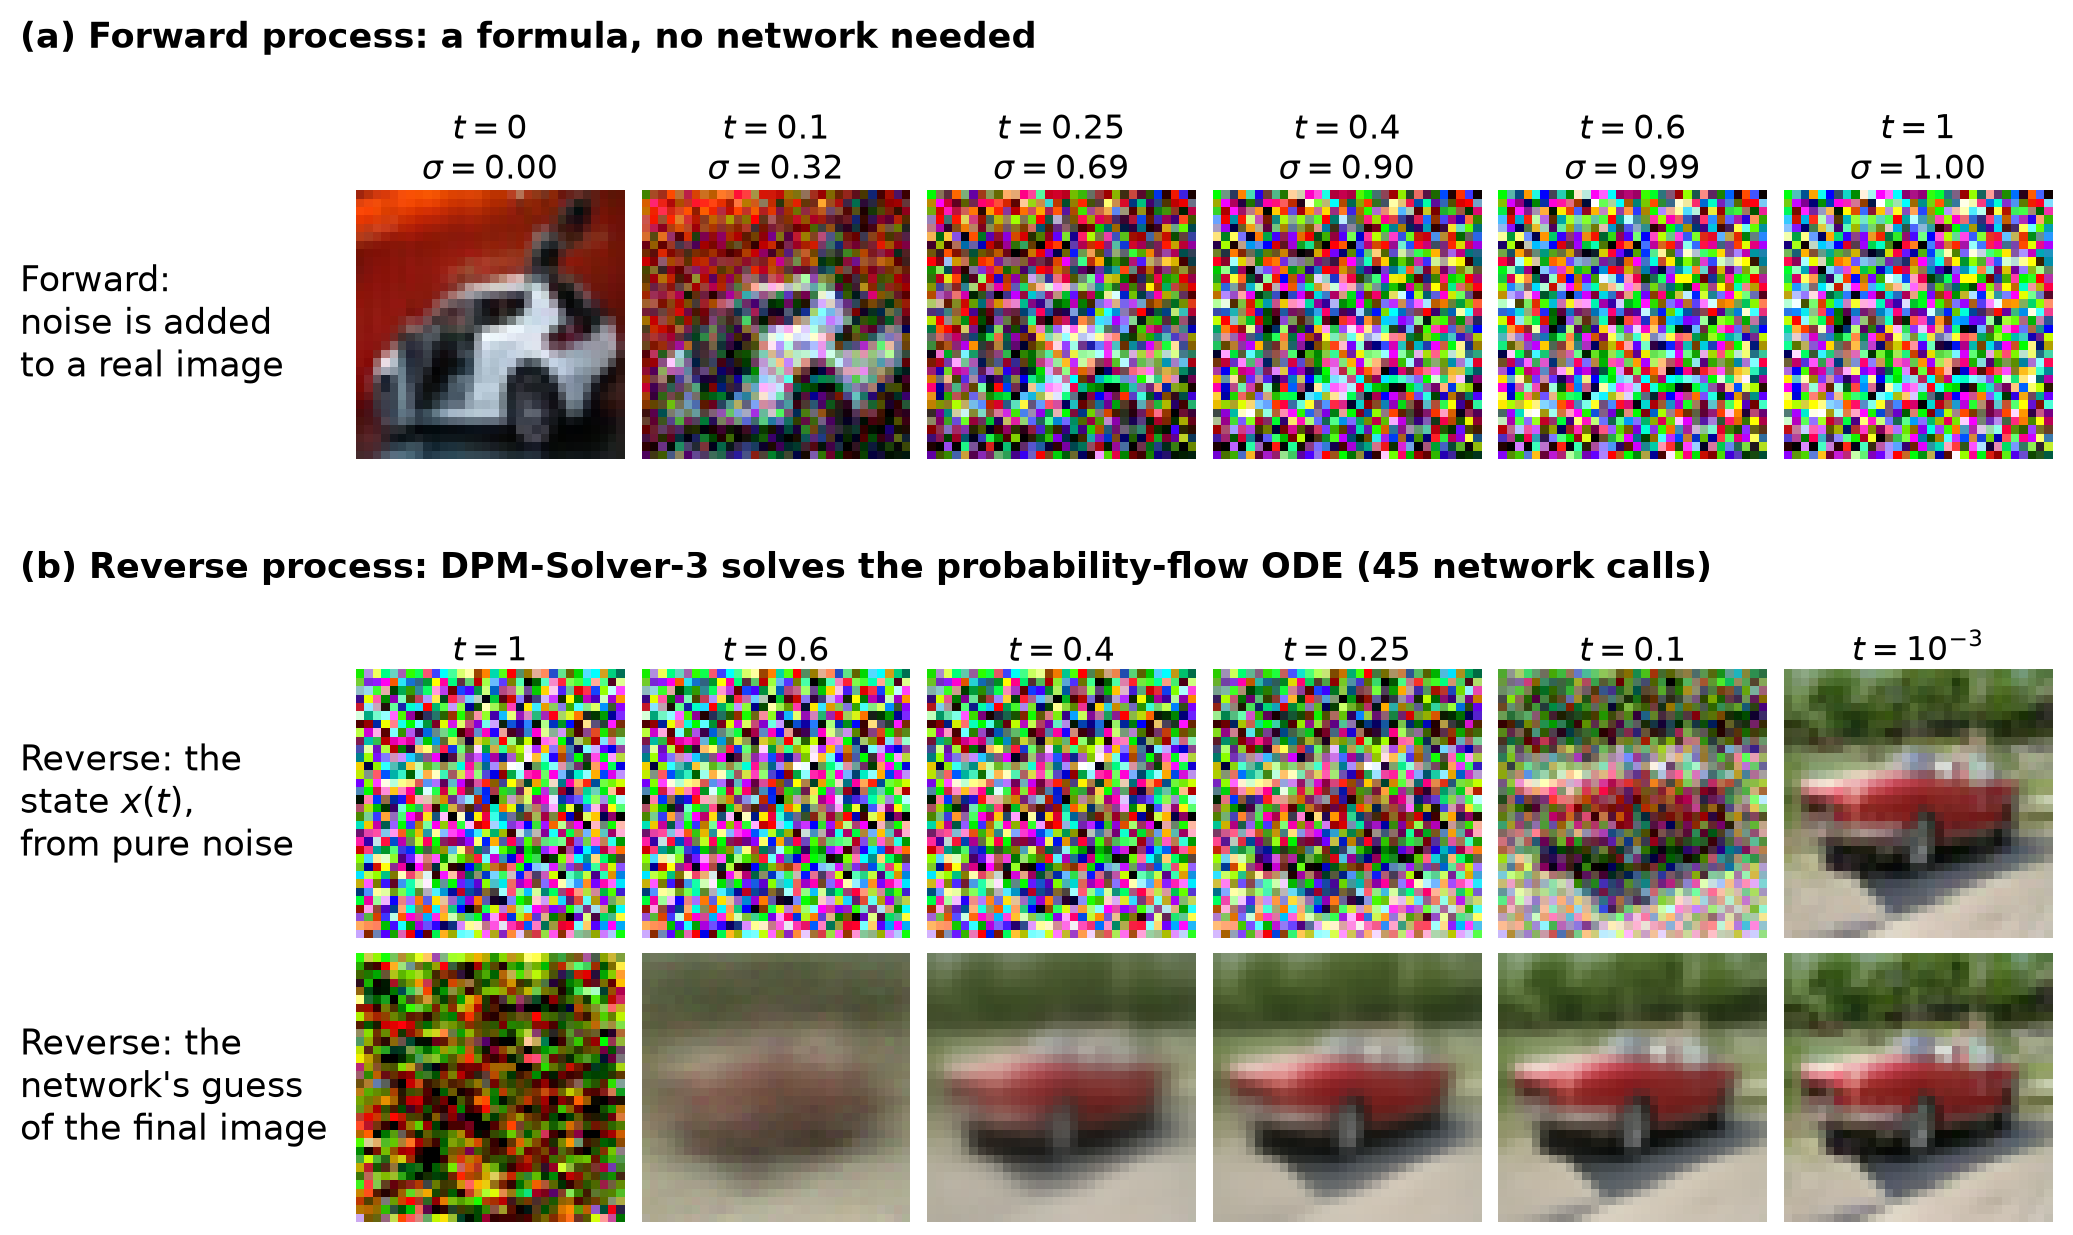
\includegraphics[width=0.94\textwidth]{diffusion_forward_reverse.png}
\caption{From noise to an image, on the CIFAR-10 checkpoint we study. (a) The
forward process mixes a real CIFAR-10 test image with Gaussian noise; at $t=1$
the image is gone. (b) Generation runs the other way: DPM-Solver-3 integrates the
probability-flow ODE from pure noise at $t=1$ to $t=10^{-3}$ with the
\texttt{google/ddpm-cifar10-32} network, in five segments that stop at the times
shown (45 network calls). Top row: the state $x(t)$ that the solver carries.
Bottom row: the network's estimate of the finished image at that moment,
$\hat x_0=(x-\sigma\eps)/\alpha$. Panel (b) is a newly generated image, not the
one in (a).}
\label{fig:diffusion}
\end{figure*}

\subsection{The base paper}

Lu et al.\ \cite{lu2022dpmsolver} observe that the probability-flow ODE is
semi-linear. Its right-hand side is a linear term in the state $x$, with a
known coefficient, plus a term that contains the network. Classical explicit
solvers such as Runge-Kutta methods \cite{hairer1993solving,butcher2016numerical}
approximate both terms. DPM-Solver integrates the linear term exactly with the
variation-of-constants formula and approximates only the network term, by a
Taylor expansion in the half log signal-to-noise ratio $\lam$. Stepping
uniformly in $\lam$ also places more steps near the data end, where the ODE
stiffens.

The paper derives solvers of order 1, 2 and 3 (DPM-Solver-1 is algebraically
the same update as DDIM \cite{song2021ddim}) and proves that DPM-Solver-$k$
converges with order $k$, under an assumption (its Assumption B.1) that the
$\lam$-derivatives of the network output exist and are continuous up to order
$k+1$. It evaluates the solvers with FID \cite{heusel2017fid} and reports good
samples in about 10 to 20 \NFE. Two further statements in the paper motivate
parts of our study. Its Section~4.2 says, citing the exponential-integrator
literature \cite{hochbruck2010exponential}, that classical explicit solvers may
become unstable at large step sizes; it does not measure a stability limit. Its
Table~6 reports, without explanation, that on the CIFAR-10 DDPM checkpoint at
about 10 \NFE\ the third-order solver scores FID 24.37 against 16.69 for the
first-order one.

\subsection{Objective of this work}

FID measures whether a set of samples resembles real data. It does not measure
how accurately a solver followed the ODE, and a sample can look plausible after
the solver has left the true trajectory. Our objective is to evaluate
DPM-Solver, and the classical solvers it is compared against, by the standards
of numerical analysis. We ask whether each solver attains its theoretical
order when measured against a known solution, how large a step each solver can
take near the stiff end before it diverges, and, once cost is counted in
\NFE, when a higher-order solver beats a lower-order one. We then put the
numerical verdict next to the image-quality verdict on the same checkpoint.

The contributions are:
\begin{itemize}
\item a three-arm design that separates DPM-Solver's two ideas, run on three
  testbeds whose references range from a closed form to a fine-grid run of a
  real network;
\item order measurements under two protocols, which show that most of the
  order shortfall seen on the real network already appears with an exact score
  at practical budgets;
\item a stability study that finds no instability on a linear problem at any
  condition number, explains why, and finds a real stability limit on a curved
  problem;
\item a crossover analysis that reproduces the paper's Table~6 anomaly at 14
  \NFE\ on the paper's own checkpoint;
\item a comparison of trajectory error and FID on the same samplers, which rank
  them in opposite orders at 10 \NFE.
\end{itemize}
All code, notebooks and results are public at
\url{https://github.com/MehemudAzad/NUMERICAL-PROJECT} \cite{ourrepo}.

% =====================================================================
\section{Methodology}
% =====================================================================

\subsection{Noise schedule and the probability-flow ODE}

We use the variance-preserving linear schedule of the base paper, with
$\beta_0=0.1$, $\beta_1=20$ and $t$ running from $T=1$ to $\tend$:
\begin{align}
\log\alpha(t) &= -\tfrac{\beta_1-\beta_0}{4}t^2-\tfrac{\beta_0}{2}t,
 \qquad \sigma(t)=\sqrt{1-\alpha(t)^2},\\
f(t) &= \tfrac{\mathrm{d}\log\alpha}{\mathrm{d}t} = -\tfrac12\beta(t),
 \qquad g^2(t)=\beta(t)=\beta_0+t(\beta_1-\beta_0).
\end{align}
The half log-SNR $\lam(t)=\log\alpha(t)-\log\sigma(t)$ decreases strictly in
$t$, from $\lam(1)\approx-5.03$ towards $+\infty$ as $t\to0$, and its inverse
has the cancellation-free form
\begin{equation}
t(\lam)=\frac{2u}{\sqrt{\beta_0^2+2(\beta_1-\beta_0)u}+\beta_0},
\qquad u=\log\!\left(e^{-2\lam}+1\right).
\end{equation}

\subsection{Three solver arms}

Write $\eps(x,t)$ for the noise-prediction model: a network in general, an
exact formula on our analytic testbeds. The same trajectory can be
discretised in three ways, and these define our three arms:
\begin{align}
\text{(A)}\;\; &\frac{\mathrm{d}x}{\mathrm{d}t}=f(t)\,x+\frac{g^2(t)}{2\sigma(t)}\,\eps(x,t),
  \label{eq:armA}\\
\text{(B)}\;\; &\frac{\mathrm{d}x}{\mathrm{d}\lam}=\hat\sigma(\lam)^2x-\hat\sigma(\lam)\,\eps\big(x,t(\lam)\big),
  \label{eq:armB}\\
\text{(C)}\;\; &x_i=\frac{\alpha_i}{\alpha_{i-1}}x_{i-1}-\sigma_i\big(e^{h_i}-1\big)\eps(x_{i-1},t_{i-1}),
  \label{eq:armC}
\end{align}
with $h_i=\lam_i-\lam_{i-1}$ and $\hat\sigma(\lam)=(1+e^{2\lam})^{-1/2}$.
Arm A applies classical steppers to Eq.~\eqref{eq:armA} on a grid uniform in
$t$. Arm B applies the same steppers to Eq.~\eqref{eq:armB}, the same ODE
written in $\lam$, on a grid uniform in $\lam$. Arm C is DPM-Solver, whose
first-order update is Eq.~\eqref{eq:armC}. Comparing A with B isolates the
change of variable, and comparing B with C isolates the exact treatment of the
linear term (Figure~\ref{fig:arms}).

The classical steppers are forward Euler, the explicit midpoint rule (RK2),
Heun's third-order method with nodes $1/3$ and $2/3$ (RK3), the classical
fourth-order Runge-Kutta method (RK4), and the two-step Adams-Bashforth method
(AB2, started with one midpoint step). The RK2 and RK3 variants are the ones in
the base paper's Appendix E.4, so arms A and B match the paper's own baselines.
For arm C we use the authors' code \cite{lu2022code}, unmodified, with one
order throughout the run (\texttt{singlestep\_fixed}), a grid uniform in $\lam$
(\texttt{logSNR}) and no final denoising step. DPM-Solver-$k$ costs $k$ \NFE\
per step. Everywhere, $e^{h}-1$ is computed with \texttt{expm1}, because the
direct form loses relative precision for the small $h$ a convergence study
needs.

\begin{figure*}[t]
\centering
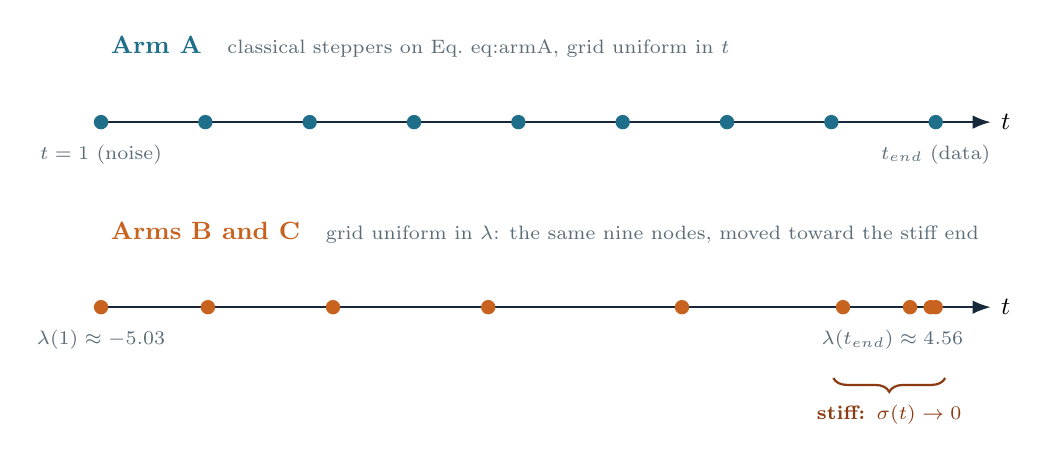
\begin{tikzpicture}[font=\small,>=Latex]
\begin{scope}[yshift=0cm]
  \node[anchor=west] at (0,.95)
    {\textcolor{armA}{\bfseries Arm A}\quad
     \textcolor{soft}{\scriptsize classical steppers on Eq.~\eqref{eq:armA}, grid uniform in $t$}};
  \draw[->,thick,ink] (0,0) -- (11.3,0) node[right,black]{$t$};
  \foreach \x in {0,1.325,2.65,3.975,5.3,6.625,7.95,9.275,10.6}
    \fill[armA] (\x,0) circle (2.6pt);
  \node[below,soft,font=\scriptsize] at (0,-.16) {$t=1$ (noise)};
  \node[below,soft,font=\scriptsize] at (10.6,-.16) {$\tend$ (data)};
\end{scope}
\begin{scope}[yshift=-2.35cm]
  \node[anchor=west] at (0,.95)
    {\textcolor{armB}{\bfseries Arms B and C}\quad
     \textcolor{soft}{\scriptsize grid uniform in $\lam$: the same nine nodes,
     moved toward the stiff end}};
  \draw[->,thick,ink] (0,0) -- (11.3,0) node[right,black]{$t$};
  \foreach \x in {0,1.357,2.946,4.917,7.378,9.423,10.274,10.536,10.6}
    \fill[armB] (\x,0) circle (2.6pt);
  \node[below,soft,font=\scriptsize] at (0,-.16) {$\lam(1)\approx-5.03$};
  \node[below,soft,font=\scriptsize] at (10.05,-.16) {$\lam(\tend)\approx4.56$};
\end{scope}
\draw[decorate,decoration={brace,amplitude=5pt,mirror},warn,thick]
      (9.30,-3.25) -- (10.72,-3.25)
      node[midway,below=6pt,warn,font=\scriptsize\bfseries]{stiff: $\sigma(t)\to0$};
\end{tikzpicture}
\caption{The three arms. All three integrate one trajectory. Arm A steps
uniformly in $t$; arms B and C step uniformly in $\lam$, which places the nodes
(computed here from the schedule) near the stiff end. Arms B and C share a grid
but not an update: arm B approximates the whole right-hand side of
Eq.~\eqref{eq:armB}, while arm C integrates its linear term exactly.}
\label{fig:arms}
\end{figure*}

\subsection{Testbeds with known answers}

Measuring error requires the correct answer, which does not exist for a real
generated image. We therefore use three testbeds (Figure~\ref{fig:tiers}).

\paragraph{Tier 1: anisotropic Gaussian.} For data drawn from
$\mathcal N(0,\operatorname{diag}(s))$ the ODE splits into $d$ independent
linear scalar ODEs, and the score and trajectory are both closed form:
\begin{equation}
\begin{gathered}
\eps^*(x,t)_j=\frac{\sigma(t)\,x_j}{v_j(t)},\qquad
v_j(t)=\alpha(t)^2s_j+\sigma(t)^2,\\
x_j(t)=x_j(T)\sqrt{v_j(t)/v_j(T)}.
\end{gathered}
\end{equation}
The stiffness parameter is the condition number $\kappa=s_{\max}/s_{\min}$.
Because the coordinates decouple, the dimension does not change the dynamics,
so we sweep $\kappa$ and keep $d$ small.

\paragraph{Tier 2: point mixture.} With data placed on $K$ points $\mu_k$, the
score stays closed form but becomes nonlinear in $x$, because the posterior mean
is a softmax over the modes:
\begin{equation}
r_k\propto w_k\exp\!\left(-\frac{\lVert x-\alpha\mu_k\rVert^2}{2\sigma^2}\right),\quad
\hat x_0=\sum_k r_k\mu_k,\quad
\eps^*=\frac{x-\alpha\hat x_0}{\sigma}.
\end{equation}
We place $K=8$ modes on a Swiss-roll curve (the testbed called \texttt{mog8}).
The responsibilities are computed with \texttt{logsumexp}, since a direct
exponentiation overflows at small $\sigma$. No closed-form trajectory exists, so
the reference is SciPy's DOP853 \cite{dormand1980family,hairer1993solving,virtanen2020scipy}.

\paragraph{Tier 3: the real network.} \texttt{google/ddpm-cifar10-32}
\cite{ddpmcifar10checkpoint,ho2020ddpm}, the DDPM checkpoint the paper uses for
its discrete-time CIFAR-10 \cite{krizhevsky2009cifar} experiments ($d=3072$).
The reference is a 201-\NFE\ DPM-Solver-3 run of the same network from the same
starting noise $x_T$, so the measurement is discretisation error and contains no
model error.

\begin{figure*}[t]
\centering
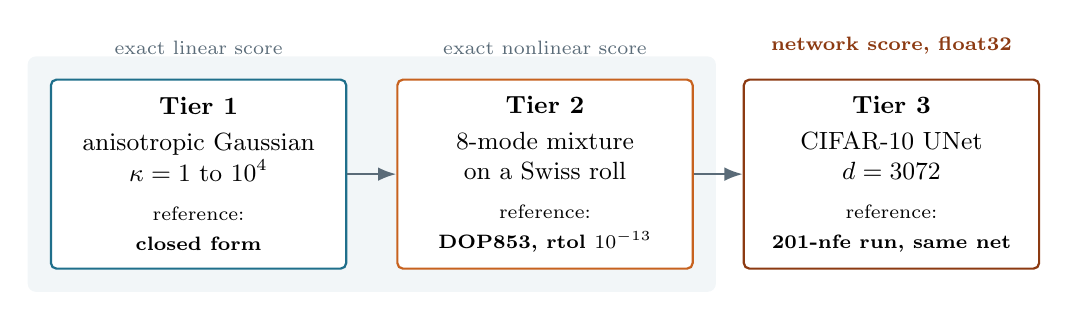
\begin{tikzpicture}[font=\small,>=Latex,
  tier/.style={draw=ink,rounded corners=2pt,minimum width=3.75cm,minimum height=2.4cm,
               align=center,inner sep=5pt,fill=white},
  lab/.style={font=\scriptsize,soft,align=center}]
\node[tier,draw=armA,thick] (t1) at (0,0)
  {\textbf{Tier 1}\\[2pt] anisotropic Gaussian\\ $\kappa = 1$ to $10^{4}$\\[3pt]
   \scriptsize reference:\\ \scriptsize\textbf{closed form}};
\node[tier,draw=armB,thick] (t2) at (4.4,0)
  {\textbf{Tier 2}\\[2pt] 8-mode mixture\\ on a Swiss roll\\[3pt]
   \scriptsize reference:\\ \scriptsize\textbf{DOP853, rtol $10^{-13}$}};
\node[tier,draw=warn,thick] (t3) at (8.8,0)
  {\textbf{Tier 3}\\[2pt] CIFAR-10 UNet\\ $d = 3072$\\[3pt]
   \scriptsize reference:\\ \scriptsize\textbf{201-\NFE\ run, same net}};
\draw[->,thick,soft] (t1) -- (t2);
\draw[->,thick,soft] (t2) -- (t3);
\node[lab,anchor=south,text width=3.6cm] at (0,1.4) {exact linear score};
\node[lab,anchor=south,text width=3.6cm] at (4.4,1.4) {exact nonlinear score};
\node[anchor=south,text width=3.6cm,font=\scriptsize\bfseries,warn,align=center]
  at (8.8,1.4) {network score, float32};
\begin{scope}[on background layer]
  \node[fit=(t1)(t2),rounded corners=3pt,fill=armA!6,inner sep=8pt] {};
\end{scope}
\end{tikzpicture}
\caption{The three testbeds. Moving right trades exactness of the reference for
realism of the problem. The shaded pair have analytic scores, so any shortfall
from theory there comes from the solver and the budget and cannot come from a
model.}
\label{fig:tiers}
\end{figure*}

\subsection{The Tier-3 schedule}

The checkpoint was trained with 1000 discrete noise levels, and the authors' code
interpolates $\log\alpha$ linearly between them. This discretised schedule
differs from the continuous one by up to $4.74\times10^{-2}$ in $\lam$ and $5.0\%$
in $f$, so reusing the continuous coefficients for arms A and B would add a
systematic error to every Tier-3 measurement. We read all coefficients from the
checkpoint's own schedule instead. Arm B needs only $t(\lam)$ and
$\hat\sigma(\lam)$, and the latter follows from $\lam=\log\alpha-\log\sigma$ and
$\alpha^2+\sigma^2=1$ for any variance-preserving schedule. Arm A needs $f$ and
$g^2$. Differentiating $\sigma^2=1-\alpha^2$ gives $\sigma'=-\alpha^2f/\sigma$,
hence
\begin{equation}
\lam'=f-\frac{\sigma'}{\sigma}=\frac{f}{\sigma^2},\qquad
f=\sigma^2\lam',\qquad g^2=-2\sigma^2\lam'=-2f.
\label{eq:vpid}
\end{equation}
We compute $\lam'$ once by a central difference and take both coefficients from
it, so $f/\lam'=\sigma^2$ holds to $1.1\times10^{-16}$. That identity is what
makes Eqs.~\eqref{eq:armA} and \eqref{eq:armB} the same ODE, and a unit test
confirms it: integrating both arms at four resolutions, the gap between them falls
from $2.5\times10^{-4}$ to $3.9\times10^{-7}$.

\subsection{Measurement procedures}

\paragraph{Order.} A measured convergence curve is straight only in its middle:
at large $h$ the asymptotic theory does not yet apply, and at small $h$ rounding
error takes over. We fit $\log(\text{error})$ against $\log h$ over every
contiguous window of at least four points and keep the window that is both
straight and wide, scored as $R^2+0.01\times(\text{width})$. We report the slope,
the window and $R^2$. On Tier 3 the reference has its own error floor (below),
and the window search can fit through it; there we also report slopes refitted
after discarding points within three times the floor.

\paragraph{Stability.} For each stepper we bisect on the number of steps, between
2 and 4096, for the coarsest grid whose output stays finite and below ten times
$\lVert x_T\rVert$, and report the corresponding largest stable step $h_{\max}$.
The bisection is checked against a synthetic linear ODE with a known stability
threshold.

\paragraph{Crossover.} To find where order 3 starts to beat order 1, we
interpolate the error curves $e_3$ of DPM-Solver-3 and $e_1$ of DPM-Solver-1
linearly in log-log space and report every sign change of $\log e_3-\log e_1$,
since the curves can cross more than once. We compare the two solvers at matched \NFE, which is the comparison in the
paper's Table~6.

\paragraph{Accuracy versus image quality.} Trajectory error is the $L_2$ distance
to the converged image, also reported per image in 8-bit gray levels. Image
quality is FID \cite{heusel2017fid}, computed with clean-fid
\cite{parmar2022cleanfid}.

% =====================================================================
\section{Implementation and experiments}
% =====================================================================

\subsection{Software and hardware}

The numerical engine is plain Python (NumPy \cite{harris2020numpy} and SciPy
\cite{virtanen2020scipy}) with no GPU code. It contains the schedule, the
testbeds, the steppers and one integrator that counts every call to the
right-hand side, so \NFE\ is measured and never inferred from a formula. The same
integrator runs all three tiers: it works on float64 NumPy arrays on Tiers 1 and 2
and on float32 PyTorch \cite{paszke2019pytorch} CUDA tensors on Tier 3, and the
probability-flow ODE is defined once, parameterised by a schedule object. Tier 3
loads the checkpoint with Diffusers \cite{vonplaten2022diffusers}. Tables are
assembled with pandas \cite{mckinney2010pandas} and figures drawn with Matplotlib
\cite{hunter2007matplotlib}. Tiers 1 and 2
run on a laptop CPU in float64; Tier 3 runs on a Kaggle NVIDIA T4 GPU
\cite{kaggle}. The repository has 129 unit tests, and \texttt{run\_all.sh}
regenerates every laptop-side result from a clean clone. Re-running it reproduced
the committed sweeps to $1.8\times10^{-15}$ and the fitted slopes to
$4.2\times10^{-5}$.

\subsection{Two protocols}

Where a convergence study is run, and at what budget, changes what it measures.
We use two settings (Table~\ref{tab:protocols}). The asymptotic protocol stays away
from the data end and starts each sweep past the solver's pre-asymptotic region,
which is the right setting for checking that an implementation has the order
promised by the theorem. The practitioner protocol is the one a user runs and the only
one affordable on Tier 3. Every comparison across tiers uses the practitioner
protocol.

\begin{table}[t]
\caption{Measurement protocols.}
\label{tab:protocols}
\small
\begin{tabular}{@{}p{1.55cm}p{2.85cm}p{3.35cm}@{}}
\toprule
Protocol & Setting & Purpose \\
\midrule
asymptotic & $t\in[0.2,1]$; $\ge 16$ to 64 \NFE, chosen per solver & test the order theorem on Tiers 1 and 2 \\
practitioner & $t\in[10^{-3},1]$; 9 to 120 \NFE & what users run; Tier 3, and Tiers 1 and 2 re-run for comparison \\
\bottomrule
\end{tabular}
\end{table}

\subsection{Parameters and data}

Table~\ref{tab:settings} lists the settings. Every run uses a fixed seed and
records a row in one shared results schema.

\begin{table}[t]
\caption{Experimental settings.}
\label{tab:settings}
\small
\begin{tabular}{@{}p{2.55cm}p{5.25cm}@{}}
\toprule
Item & Value \\
\midrule
Schedule & VP linear, $\beta_0=0.1$, $\beta_1=20$, $T=1$ \\
Tier 1 & $d=3$; $\kappa\in\{1,10,10^2,10^3,10^4\}$, stability stress test to $10^8$ \\
Tier 2 & \texttt{mog8}: 8 equal-weight modes on a Swiss roll \\
Tier 2 reference & DOP853, rtol $10^{-13}$, atol $10^{-14}$; rerun at $10^{-11}$ agrees to $6.9\times10^{-13}$ \\
Tier 3 batch & 64 images, seed 0, float32 \\
Tier 3 references & DPM-Solver-3 at 201 \NFE; 300 \NFE\ for the floor; $\tend\in\{2,5,10\}\times10^{-3}$ for truncation \\
Tier 3 budgets & 10, 12, 15, 20, 30, 50, 80, 120 \NFE \\
Sample grid & 6 samplers $\times$ 5 budgets on 8 noises; 64 images per sampler for per-image error \\
FID & 5{,}000 samples per setting, clean-fid, \texttt{legacy\_tensorflow}, CIFAR-10 training statistics \\
FID floor & real CIFAR-10 test images: three draws each of 1{,}000, 2{,}000 and 5{,}000; the full 10{,}000 once \\
\bottomrule
\end{tabular}
\end{table}

The benchmark is the base paper itself: its Table~6 (FID of DPM-Solver-1, -2, -3
and DPM-Solver-fast on this checkpoint, $\epsilon=10^{-3}$) and its Table~4 (DDIM
on the same checkpoint). Two samplers that our sweeps had not used are added for
the FID comparison because the paper uses them: DPM-Solver-fast, which mixes orders
1 to 3 to spend the budget exactly, and DDIM on its quadratic time grid.

\subsection{Validation}
\label{sec:validation}

The paper shows that DDIM and DPM-Solver-1 are algebraically the same update, so
two independent implementations must agree to machine precision. Ours agree to
$5.5\times10^{-16}$, and DPM-Solver-1 measures as order $0.99$; nothing downstream
was run before this check passed. The Tier-1 closed form satisfies the ODE to about
$10^{-11}$ and matches an independent DOP853 integration to $10^{-12}$, and our
continuous schedule agrees with the one in the authors' code to $10^{-11}$, so all
three arms share one schedule.

% =====================================================================
\section{Results and discussion}
% =====================================================================

We ran seven experiments. Table~\ref{tab:summary} lists what each one asks and what
it found; the subsections below give the measurements behind each row.

\begin{table*}[t]
\caption{The seven experiments at a glance: the question each one asks, and the
answer the measurements give.}
\label{tab:summary}
\small
\begin{tabular}{@{}r@{\hspace{6pt}}p{2.9cm}p{4.0cm}p{7.6cm}l@{}}
\toprule
& Experiment & Question & Result & Section \\
\midrule
1 & DDIM $\equiv$ DPM-Solver-1 & Is our implementation exact? &
  The two updates agree to $5.5\times10^{-16}$; DPM-Solver-1 measures order 0.99. &
  \ref{sec:validation} \\
2 & Convergence order & Does the error fall at the textbook rate? &
  With an exact score and small steps, every solver is within 0.094 of theory. At
  10 to 120 \NFE\ down to $t=10^{-3}$ the order misses theory by up to 1.91 with an
  exact score and 2.79 on the network. & \ref{sec:order}, \ref{sec:practical} \\
3 & Stability near $t\to0$ & Do large steps diverge near the data? &
  Linear testbed: never, up to $\kappa=10^8$. Curved testbed: RK4 in $t$ is limited
  to $h\le0.1998$. Stepping in $\lam$: never. & \ref{sec:stability} \\
4 & Crossover at equal cost & When does order 3 beat order 1? &
  From 5.1, 9.2 and 14.1 \NFE\ on Tiers 1, 2 and 3; the paper's Table~6 puts it
  between 10 and 12. & \ref{sec:crossover} \\
5 & Change of variable (A vs B) & What does stepping in $\lam$ buy? &
  RK4's error falls $48\times$, $8551\times$ and $10.6\times$ on the three tiers; for
  Euler and RK2 the effect is mixed. & \ref{sec:reparam} \\
6 & Exact linear part (B vs C) & When does it help? &
  On concentrated data (ahead at 83 to 100\% of points for $s<10^{-2}$). For data as
  spread out as the noise ($s=1$) classical steppers are exact and DPM-Solver-1 is
  not. & \ref{sec:split} \\
7 & Image quality vs accuracy & Is the best-looking sampler the most accurate? &
  No. At 10 \NFE\ FID and distance to the converged image rank the samplers in
  exactly opposite order (rank correlation $-1.00$; $+0.60$ at 20 \NFE). Sample size
  explains about half of the gap to the paper's FIDs. & \ref{sec:fid} \\
\bottomrule
\end{tabular}
\end{table*}

\subsection{Order with an exact score}
\label{sec:order}

Under the asymptotic protocol every solver in every arm reaches its theoretical
order (Table~\ref{tab:order12}, Figure~\ref{fig:errh}). The largest deviation is
$0.094$ on Tier 1 and $0.084$ on Tier 2, with mean $R^2$ of $0.99992$ and $0.99996$,
and moving from the linear to the curved testbed shifts no slope by more than
$0.059$. Both testbeds have analytic scores, so Assumption B.1 holds and the
theorem's conclusion holds with it. The result also confirms that the published
code, driven by an exact oracle, implements the method correctly.

\begin{figure}[t]
\centering
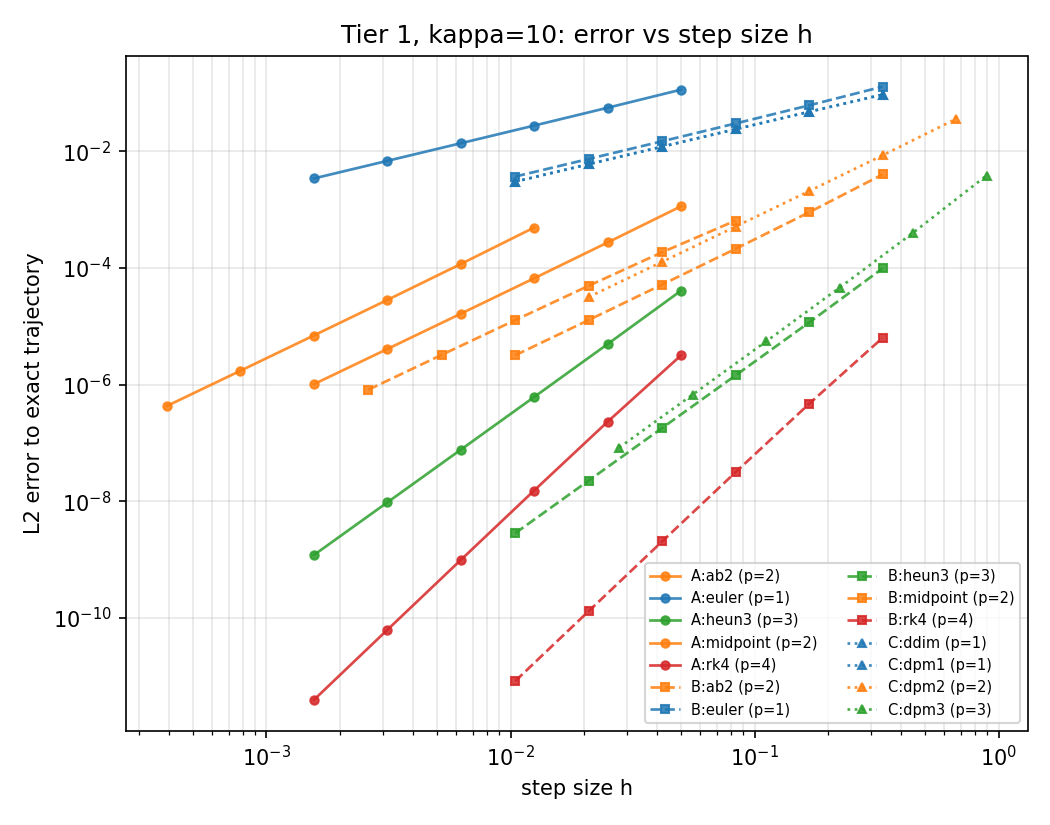
\includegraphics[width=\columnwidth]{05_error_vs_h.png}
\caption{Tier 1 ($\kappa=10$), asymptotic protocol: error against step size for
every solver in every arm. The slope of each line is its measured order
(Table~\ref{tab:order12}). DDIM and DPM-Solver-1 lie on top of each other.}
\label{fig:errh}
\end{figure}

\paragraph{Cost per \NFE.} Order is defined per step, but a step of RK4 costs four
network calls and a step of DPM-Solver-$k$ costs $k$. Figure~\ref{fig:frontier}
puts the Tier-1 errors on a common \NFE\ axis. In the asymptotic regime the higher
order pays for its extra calls: RK4 in $t$ is 21 times more accurate than
DPM-Solver-3 at 64 \NFE\ and 121 times at 512. The advantage the paper claims for
DPM-Solver lies at 10 to 20 \NFE, which these sweeps never visit. Tier 3 does, and
there DPM-Solver-3 beats RK4 per \NFE\ from 16 to 120 \NFE\ (Figure~\ref{fig:t3}).

\begin{figure}[t]
\centering
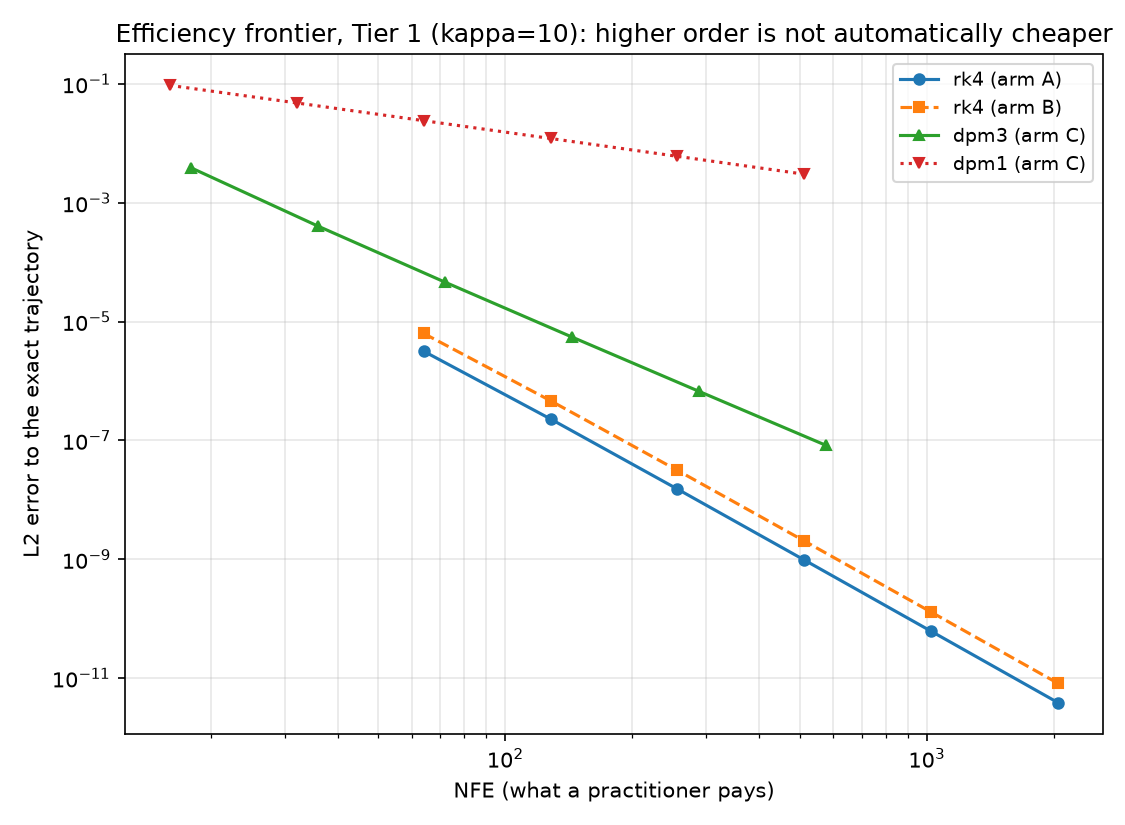
\includegraphics[width=\columnwidth]{10_efficiency_frontier.png}
\caption{Tier 1 ($\kappa=10$), asymptotic protocol: error against measured \NFE,
the cost a user pays. RK4 in either variable stays below DPM-Solver-3 at every
shared budget.}
\label{fig:frontier}
\end{figure}

\begin{table}[t]
\caption{Measured order with an exact score, asymptotic protocol.}
\label{tab:order12}
\small
\begin{tabular}{@{}llcccc@{}}
\toprule
Arm & Solver & $p$ & Tier 1 & Tier 2 & max $|\Delta|$ \\
\midrule
A & Euler    & 1 & 1.012 & 1.012 & 0.012 \\
A & midpoint & 2 & 2.028 & 2.031 & 0.031 \\
A & Heun3    & 3 & 3.014 & 2.999 & 0.014 \\
A & RK4      & 4 & 3.938 & 3.997 & 0.062 \\
A & AB2      & 2 & 2.033 & 1.988 & 0.033 \\
\midrule
B & Euler    & 1 & 1.023 & 1.023 & 0.023 \\
B & midpoint & 2 & 2.057 & 2.055 & 0.057 \\
B & Heun3    & 3 & 3.015 & 3.024 & 0.024 \\
B & RK4      & 4 & 3.921 & 3.965 & 0.079 \\
B & AB2      & 2 & 1.935 & 1.975 & 0.065 \\
\midrule
C & DDIM     & 1 & 0.994 & 0.996 & 0.006 \\
C & DPM-1    & 1 & 0.994 & 0.996 & 0.006 \\
C & DPM-2    & 2 & 2.028 & 2.018 & 0.028 \\
C & DPM-3    & 3 & 3.094 & 3.084 & 0.094 \\
\bottomrule
\end{tabular}
\end{table}

\begin{table*}[t]
\caption{Measured order under both protocols. Floor-excl.\ refits Tier 3 after
discarding points within three times the reference floor.}
\label{tab:order3}
\small
\begin{tabular}{@{}llc cc ccc c@{}}
\toprule
 & & & \multicolumn{2}{c}{asymptotic} & \multicolumn{4}{c}{practitioner ($\tend=10^{-3}$, 9 to 120 \NFE)} \\
\cmidrule(lr){4-5}\cmidrule(lr){6-9}
Arm & Solver & $p$ & Tier 1 & Tier 2 & Tier 1 & Tier 2 & Tier 3 & floor-excl. \\
\midrule
A & Euler    & 1 & 1.012 & 1.012 & 0.871 & 1.269 & 0.842 & 0.842 \\
A & midpoint & 2 & 2.028 & 2.031 & 2.403 & 1.485 & 1.525 & 1.500 \\
A & RK4      & 4 & 3.938 & 3.997 & 3.297 & 2.093 & 1.210 & 1.210 \\
\midrule
B & Euler    & 1 & 1.023 & 1.023 & 1.073 & 1.191 & 0.746 & 0.746 \\
B & midpoint & 2 & 2.057 & 2.055 & 1.786 & 2.385 & 1.603 & 1.603 \\
B & RK4      & 4 & 3.921 & 3.965 & 4.829 & 4.523 & 2.231 & $1.099^{\dagger}$ \\
\midrule
C & DPM-1    & 1 & 0.994 & 0.996 & 0.958 & 1.325 & 0.813 & 0.813 \\
C & DPM-2    & 2 & 2.028 & 2.018 & 2.100 & 2.455 & 2.191 & 2.244 \\
C & DPM-3    & 3 & 3.094 & 3.084 & 3.492 & 4.214 & 2.473 & \textbf{2.995} \\
\midrule
\multicolumn{3}{@{}l}{worst $|\text{slope}-p|$} & 0.094 & 0.084 & 0.83 & 1.91 & 2.79 & \\
\bottomrule
\end{tabular}

\smallskip
{\footnotesize $^{\dagger}$Two of eight points lie on the floor; the six left are
mostly pre-asymptotic, so neither Tier-3 value is reliable for B/RK4.}
\end{table*}

\subsection{Order at practical budgets}
\label{sec:practical}

Table~\ref{tab:order3} repeats the measurement under the practitioner protocol on
all three tiers. With an exact score and nothing else changed except the interval
and the budget, the slopes scatter on both sides of theory by up to $1.91$: RK4 in
$t$ on Tier 2 measures $2.09$ and RK4 in $\lam$ measures $4.52$. At 9 to 120 \NFE,
integrating down to $10^{-3}$, no solver is in the asymptotic regime its order
describes, with or without a network. The exact-score Tier 2 already shows $68\%$
of the network's worst gap ($1.91$ of $2.79$; Figure~\ref{fig:matched}).

The network adds a further downward shift, largest for the high-order steppers:
measured against the matched Tier-2 control, RK4 in $t$ falls from $2.09$ to $1.21$,
RK4 in $\lam$ from $4.52$ to $2.23$ and DPM-Solver-3 from $4.21$ to $2.47$.
DPM-Solver-3's value is affected by the reference floor: discarding the one sweep
point that reaches it gives $2.995$, close to its theoretical order. Curves far
above the floor, such as RK4 in $t$ at twelve times the floor, do not change.

An earlier version of our analysis attributed the Tier-3 shortfall to the network
violating Assumption B.1. The matched control does not support that. The
assumption only requires the $\lam$-derivatives of $\eps$ to exist and be
continuous, and this UNet, built from SiLU activations \cite{elfwing2018silu},
normalisation and sinusoidal time embeddings, is a smooth function of its inputs.
A network can make those derivatives large, which moves the start of the
asymptotic regime to smaller steps than any practical budget reaches.

\begin{figure}[t]
\centering
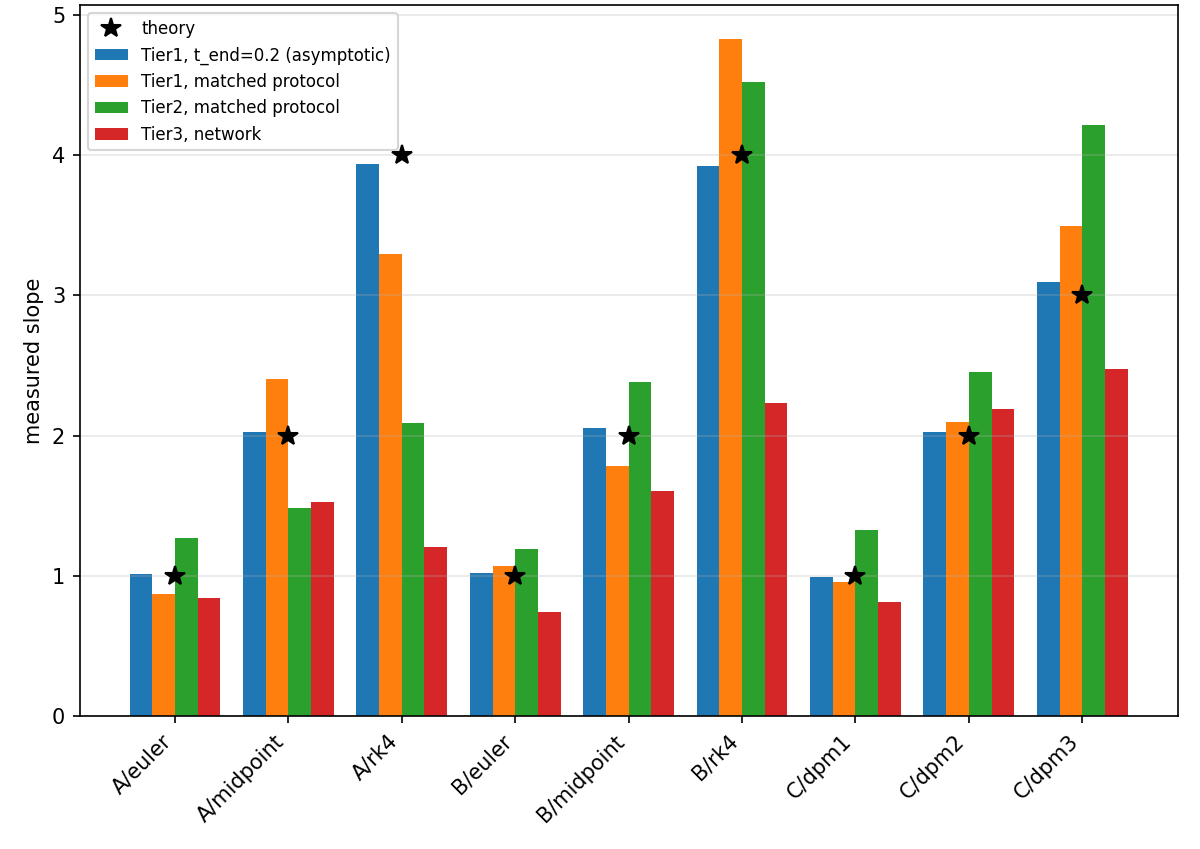
\includegraphics[width=\columnwidth]{12_matched_protocol.png}
\caption{Measured slopes against theory (stars). Tier 1 under the asymptotic
protocol, Tiers 1 and 2 under the practitioner protocol, and Tier 3. The large
departures appear with an exact score once the protocol matches Tier 3's.}
\label{fig:matched}
\end{figure}

\subsection{Stability}
\label{sec:stability}

\paragraph{Linear testbed.} For every $\kappa$ from 1 to $10^4$, every stepper in
both arms is stable on the coarsest grid tried (two steps), and the stress test to
$\kappa=10^8$ and $\tend=10^{-6}$ changes nothing. The cause is structural. On a
uniform-$t$ grid the node nearest the boundary is at $\tend+h$, and the stability
product $h\,J(\tend+h)$, with $J$ the local Jacobian, never exceeds about $0.9$,
below explicit Euler's threshold of 2. Near the boundary $\sigma(t)^2\approx\beta_0t$,
so the growth of the local rate and the shrinking distance to $\tend$ almost cancel,
and for $s_{\min}\ll\sigma^2$ the rate is capped by $\sigma^2$ and does not depend
on $\kappa$.

\paragraph{Curved testbed.} On Tier 2 the Jacobian has no such cancellation
(Figure~\ref{fig:stab}). As $\sigma\to0$ the posterior weights switch more sharply
between modes, and at $t=10^{-3}$ the spectral norm of the arm-A Jacobian is 545,
against 0.54 on Tier 1. RK4 in $t$ now has a real limit, $h_{\max}=0.1998$: it is
stable from 5 steps and diverges at 2 to 4. A stricter divergence rule gives the
same limit. RK4 is the only arm-A stepper whose last stage evaluates the right-hand
side at the end of the step, which on the final step is $\tend$, where the Jacobian
peaks. In arm B every stepper is stable at every grid tried.

The paper's Section~4.2 statement therefore holds in a narrower form: explicit
steppers in $t$ can become unstable near the data, the instability comes from the
curvature of the data distribution and does not depend on $\kappa$, and the $\lam$
reparameterisation removes it.

\begin{figure}[t]
\centering
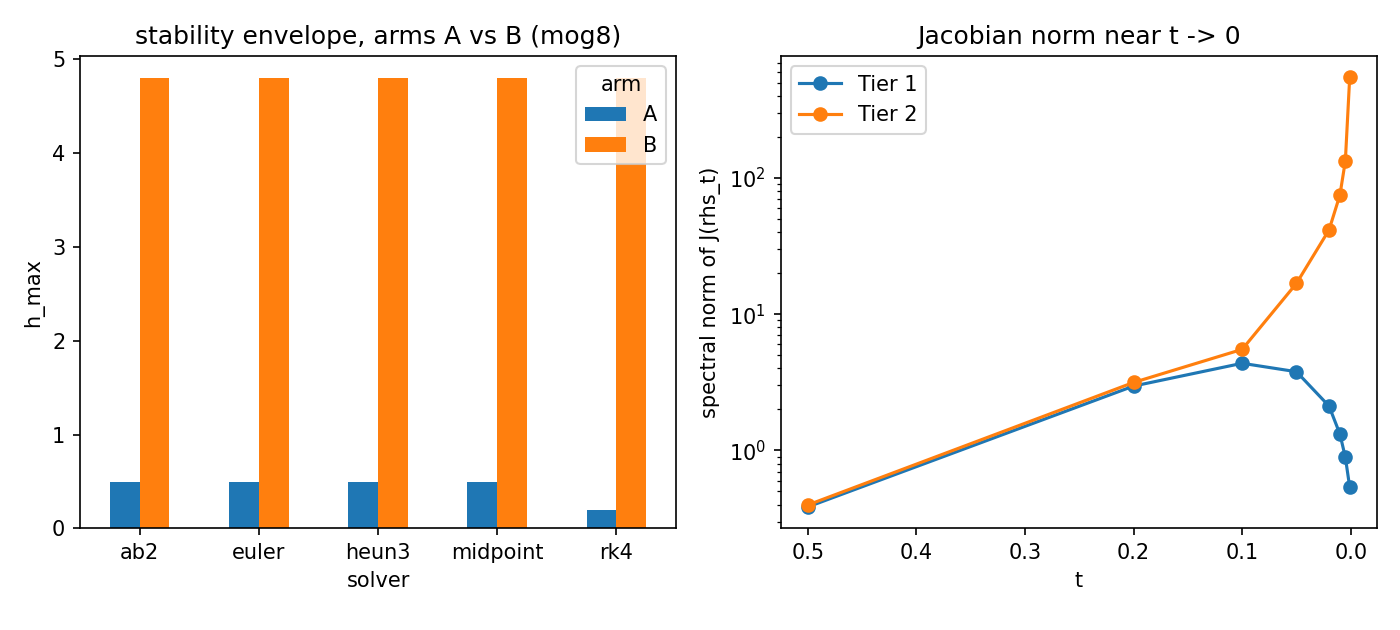
\includegraphics[width=\columnwidth]{stability_two_panels.png}
\caption{Stability on Tier 2. Left: largest stable step per stepper; bars at 0.4995
(in $t$) and 4.79 (in $\lam$) are the coarsest grids tried, so those steppers never
diverged, and only arm-A RK4 is limited. Right: spectral norm of the arm-A Jacobian
along the trajectory; Tier 1 turns down near $t\to0$ while Tier 2 climbs to 545.}
\label{fig:stab}
\end{figure}

\begin{figure*}[t]
\centering
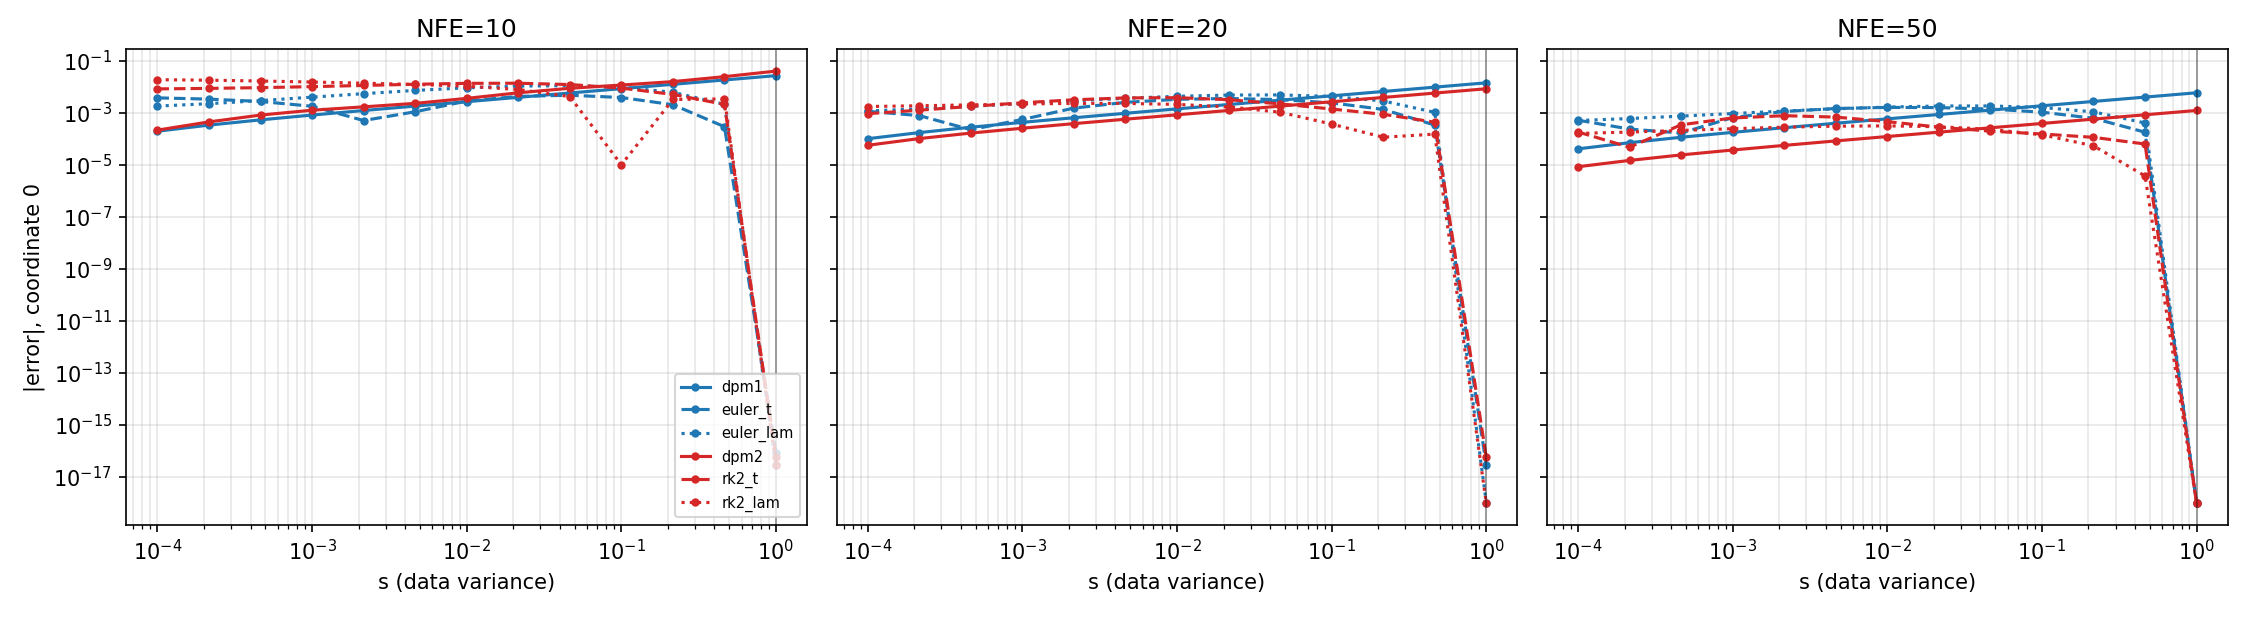
\includegraphics[width=0.92\textwidth]{12_split_benefit.png}
\caption{Error on one Gaussian coordinate of data variance $s$ at 10, 20 and 50
\NFE. Solid lines: DPM-Solver-1 and -2. Dashed and dotted: classical steppers of the
same order in $t$ and in $\lam$. DPM-Solver leads for small $s$; at $s=1$ the
classical right-hand side cancels and those steppers reach machine precision.}
\label{fig:split}
\end{figure*}

\subsection{What the change of variable buys}
\label{sec:reparam}

Arms A and B integrate the same ODE, so their ratio of errors measures the change
of variable alone (Table~\ref{tab:reparam}). For RK4 the $\lam$ form is more
accurate on every tier once the run reaches the data end, by factors of 48, 8551
and 10.6. Under the asymptotic protocol, which stops at $t=0.2$, the factors are
$0.47$ and $1.77$, which is why the analytic tiers first appeared indifferent to it.
A grid uniform in $t$ leaves one long final step across the region where
$\sigma\to0$, and RK4's stages sample that region. For Euler and RK2 the effect is
mixed: the $\lam$ form helps on Tier 2 by factors of 10 to 33 and is slightly worse
on Tier 1 and on the network.

\begin{table}[t]
\caption{Error of arm A divided by error of arm B at the largest shared \NFE.
Values above 1 favour the $\lam$ grid.}
\label{tab:reparam}
\small
\begin{tabular}{@{}llccc@{}}
\toprule
Protocol & Tier & Euler & RK2 & RK4 \\
\midrule
asymptotic   & 1 & 0.93 & 0.32 & 0.47 \\
             & 2 & 0.92 & 0.39 & 1.77 \\
\midrule
practitioner & 1 & 0.69 & 0.85 & \textbf{48.4} \\
             & 2 & 9.92 & 33.1 & \textbf{8551} \\
             & 3 & 0.63 & 0.56 & \textbf{10.6} \\
\bottomrule
\end{tabular}
\end{table}

\subsection{When the exact linear treatment helps}
\label{sec:split}

The two analytic tiers disagree about DPM-Solver's split. On Tier 1 ($\kappa=10$),
DPM-Solver-1 and -2 lose to the classical stepper of the same order at every budget
from 10 to 120 \NFE: at 20 \NFE, DPM-Solver-2 errs by $0.133$, RK2 in $t$ by $0.034$
and RK2 in $\lam$ by $0.0089$. On Tier 2, at 12 \NFE, DPM-Solver-2 errs by $0.084$
against $0.23$ (RK2 in $\lam$) and $0.34$ (RK2 in $t$).

The difference is how concentrated the data is. For data concentrated at a point
($s\to0$), $\eps=x/\sigma$ is constant along the exact path, and substituting
$e^{h}=\alpha_i\sigma_{i-1}/(\sigma_i\alpha_{i-1})$ into Eq.~\eqref{eq:armC} gives
$x_i=(\sigma_i/\sigma_{i-1})x_{i-1}$, the exact solution. For data as spread out as
the noise ($s=1$), the right-hand side of Eq.~\eqref{eq:armA} is identically zero and
every classical stepper is exact, while $\eps=\hat\sigma(\lam)x$ still varies and
DPM-Solver-1 is not. Sweeping $s$ between the two (Figure~\ref{fig:split}), at 20
\NFE\ and $s<10^{-2}$ DPM-Solver-1 beats Euler in $t$ at 83\% of points and
DPM-Solver-2 beats RK2 in $t$ at all of them; at $s=1$ the classical steppers are
exact to $10^{-16}$ while DPM-Solver-1 errs by $5.9\times10^{-3}$. Natural images
have a rapidly decaying pixel covariance spectrum, which puts most directions at
the concentrated end and is consistent with DPM-Solver's success on them. We have
not measured that spectrum.

\subsection{The crossover and Table 6}
\label{sec:crossover}

What is held fixed matters. Compared at the same step size, which gives
DPM-Solver-3 three times the budget of DPM-Solver-1, the two curves cross at 4.4 to
5.0 \NFE\ on Tier 1, flat across five decades of $\kappa$, and at 8.9 on Tier 2. The
fair comparison, and the practical one, holds the budget fixed, so everything below
is at matched \NFE.

On this checkpoint the paper's Table~6 gives DPM-Solver-3 an FID of 24.37 (at an
actual 9 \NFE) against 16.69 for DPM-Solver-1 at 10 \NFE, and the order reverses by
12 \NFE\ (8.20 against 13.63). With exact answers and a continuous budget we can
locate the crossing (Table~\ref{tab:cross}, Figure~\ref{fig:cross}). On the real
network, at matched \NFE, DPM-Solver-3 overtakes DPM-Solver-1 at 14.1 \NFE, close to
the paper's 10 to 12, with a trajectory-error metric instead of FID. The first
crossing moves later as the problem gets harder: 5.1 on the linear Gaussian, 9.2 on
the mixture and 14.1 on the network. This fits a pre-asymptotic explanation. At 9
\NFE\ DPM-Solver-3 takes only three steps, and with steps that large its third-order
correction increases the error. The larger the higher $\lam$-derivatives of $\eps$
along the path, the smaller the step must be before the correction helps. Our own
FIDs show the same reversal: DPM-Solver-3 scores 143 at 9 \NFE\ against 44.9 for
DPM-Solver-1 at 10, and 18.7 at 18 \NFE\ against 27.0 at 20.

\begin{table}[t]
\caption{\NFE\ at which DPM-Solver-3 and DPM-Solver-1 cross, at matched \NFE,
practitioner protocol.}
\label{tab:cross}
\small
\begin{tabular}{@{}lll@{}}
\toprule
Testbed & Crossings & Note \\
\midrule
Tier 1, Gaussian & 5.1 & one crossing \\
Tier 2, \texttt{mog8} & 9.2, 14.2, 17.3 & order 3 stays ahead from 17.3 \\
Tier 3, CIFAR-10 & \textbf{14.1} & paper's checkpoint \\
Paper, Table 6 (FID) & 10 to 12 & same checkpoint \\
\bottomrule
\end{tabular}
\end{table}

\begin{figure}[t]
\centering
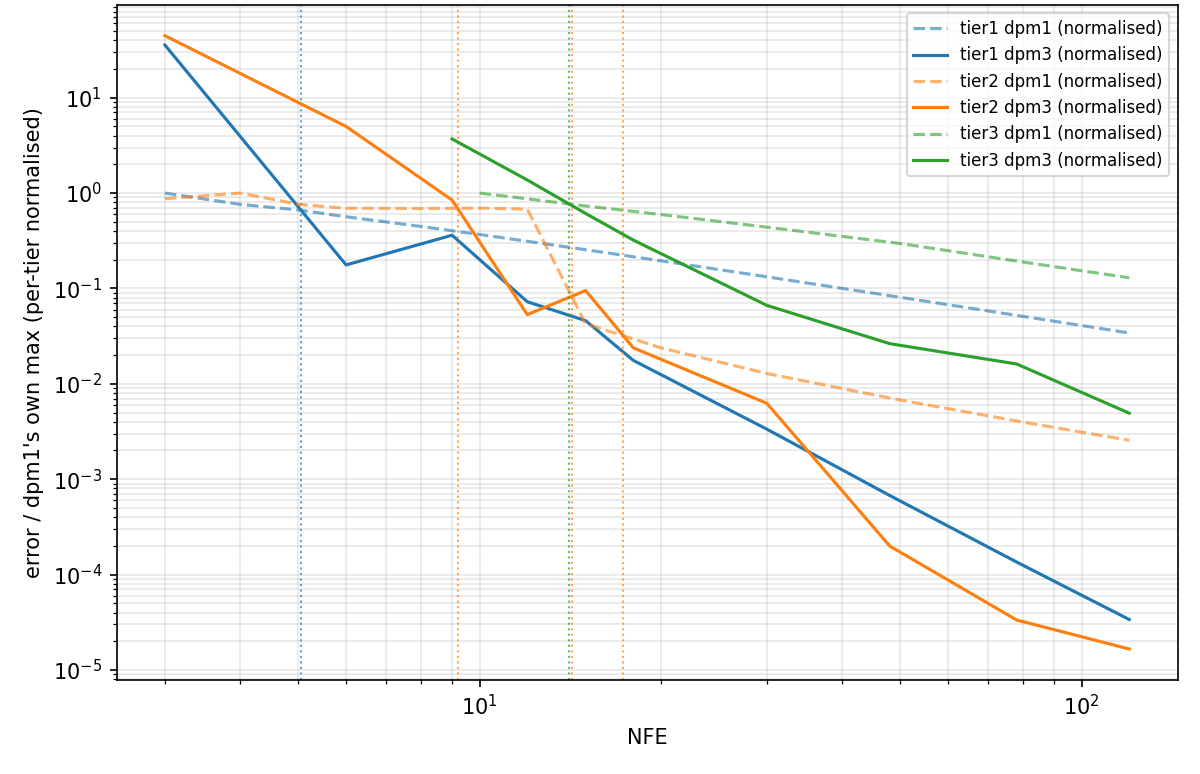
\includegraphics[width=\columnwidth]{12_crossover_matched_nfe.png}
\caption{DPM-Solver-3 (solid) against DPM-Solver-1 (dashed) at matched \NFE, each
tier normalised by its own DPM-Solver-1 maximum. Dotted verticals mark crossings.}
\label{fig:cross}
\end{figure}

\begin{figure}[t]
\centering
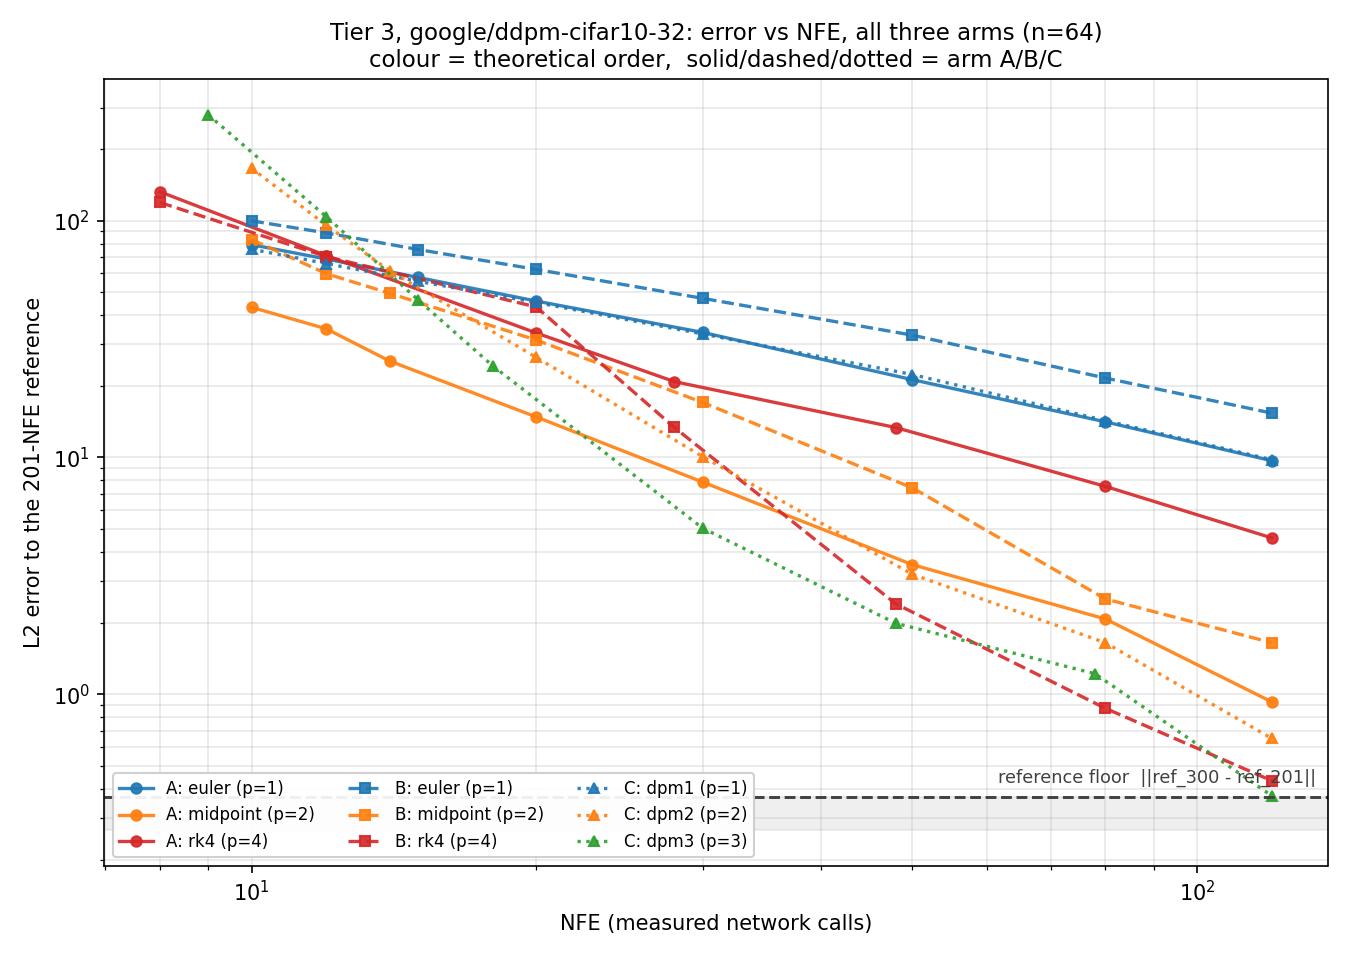
\includegraphics[width=\columnwidth]{09_tier3_error_vs_nfe.png}
\caption{Tier 3: error against measured \NFE\ for all nine solver and arm
combinations. The dashed horizontal line is the reference floor
$\lVert x_{300}-x_{201}\rVert$.}
\label{fig:t3}
\end{figure}

\subsection{Tier-3 error and its components}

Figure~\ref{fig:t3} shows Tier-3 error against \NFE\ for all nine solver and arm
combinations. Total error on Tier 3 has three parts, and each can be measured
without the true score (Table~\ref{tab:decomp}, Figure~\ref{fig:decomp}). The floor, the disagreement between
two references, is $0.368$ in total, or $8\times10^{-4}$ relative to
$\lVert x\rVert\approx\sqrt{3072}$, which matches the expected float32 precision of
about $10^{-3}$. Stopping at $\tend=2\times10^{-3}$ instead of $10^{-3}$ moves the
result by $1.53$, more than DPM-Solver-3's whole discretisation error at 78 \NFE\
($1.22$). Beyond that budget, extra network calls reduce a component that the choice
of $\tend$ already outweighs. The paper's Table~4 shows the same effect in FID: the
type-2 DPM-Solver scores 4.39 at 15 \NFE\ and 5.52 at 20.

\begin{figure}[t]
\centering
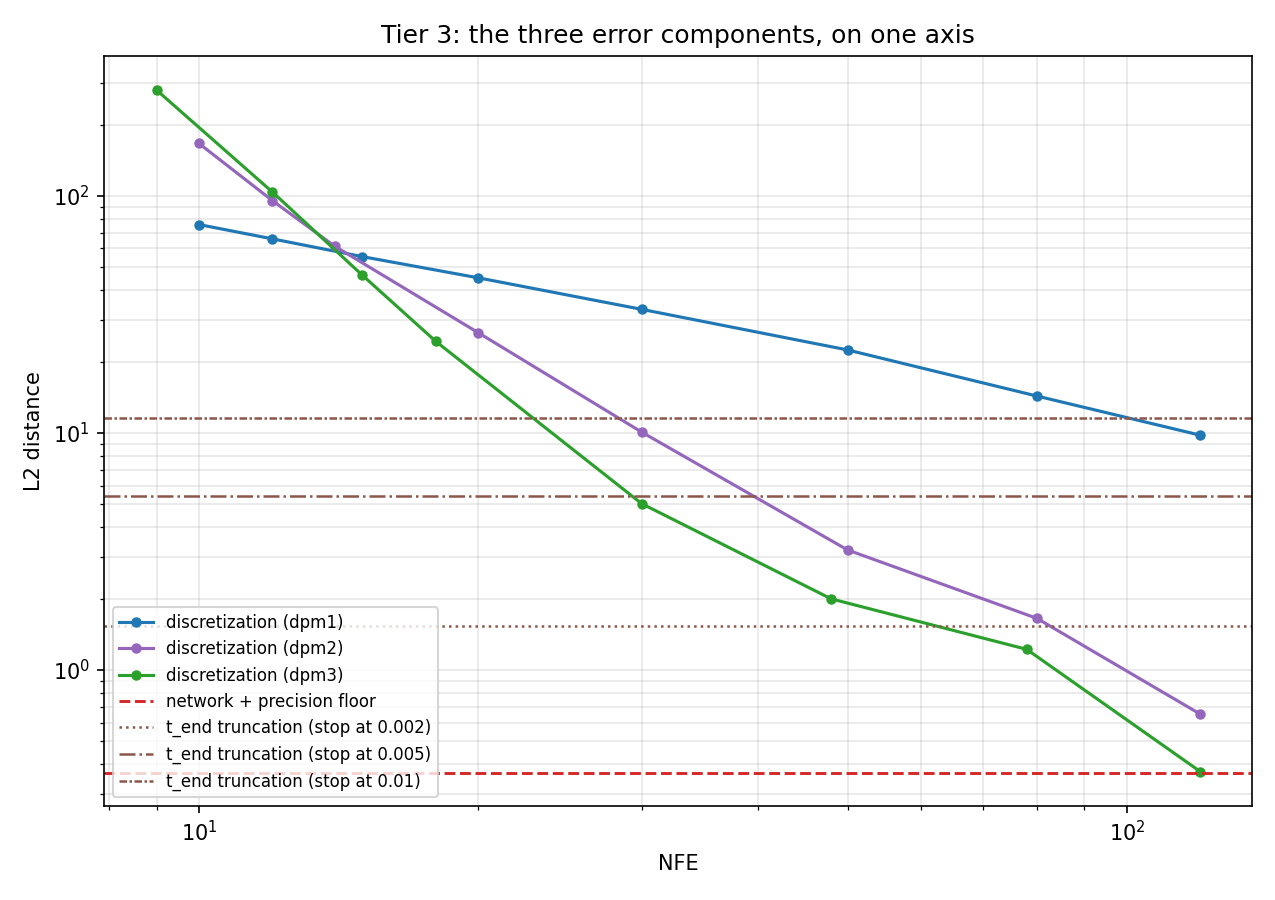
\includegraphics[width=\columnwidth]{09_tier3_decomposition.png}
\caption{The three Tier-3 error components on one axis: discretisation error of
DPM-Solver-1, -2 and -3 against \NFE, the $\tend$ truncation for stopping at
$2$, $5$ and $10\times10^{-3}$ (horizontal lines), and the reference floor (red,
dashed). Once a discretisation curve falls below a truncation line, the choice of
$\tend$ matters more than further network calls.}
\label{fig:decomp}
\end{figure}

\begin{table}[t]
\caption{The three components of Tier-3 error.}
\label{tab:decomp}
\small
\begin{tabular}{@{}p{2.1cm}p{3.15cm}p{2.3cm}@{}}
\toprule
Component & Measured as & Value \\
\midrule
discretisation & $\lVert x_N-x_{\text{ref}}\rVert$, DPM-Solver-3 & 279.6 at 9 \NFE\ to 0.37 at 120 \\
$\tend$ truncation & $\lVert x_{\text{ref}}(\tend)-x_{\text{ref}}(10^{-3})\rVert$ & 1.53, 5.43, 11.56 at $\tend=2,5,10\times10^{-3}$ \\
network and precision floor & $\lVert x_{300}-x_{201}\rVert$ & 0.368 \\
\bottomrule
\end{tabular}
\end{table}

\begin{figure*}[t]
\begin{minipage}[t]{0.50\textwidth}\vspace{0pt}\centering
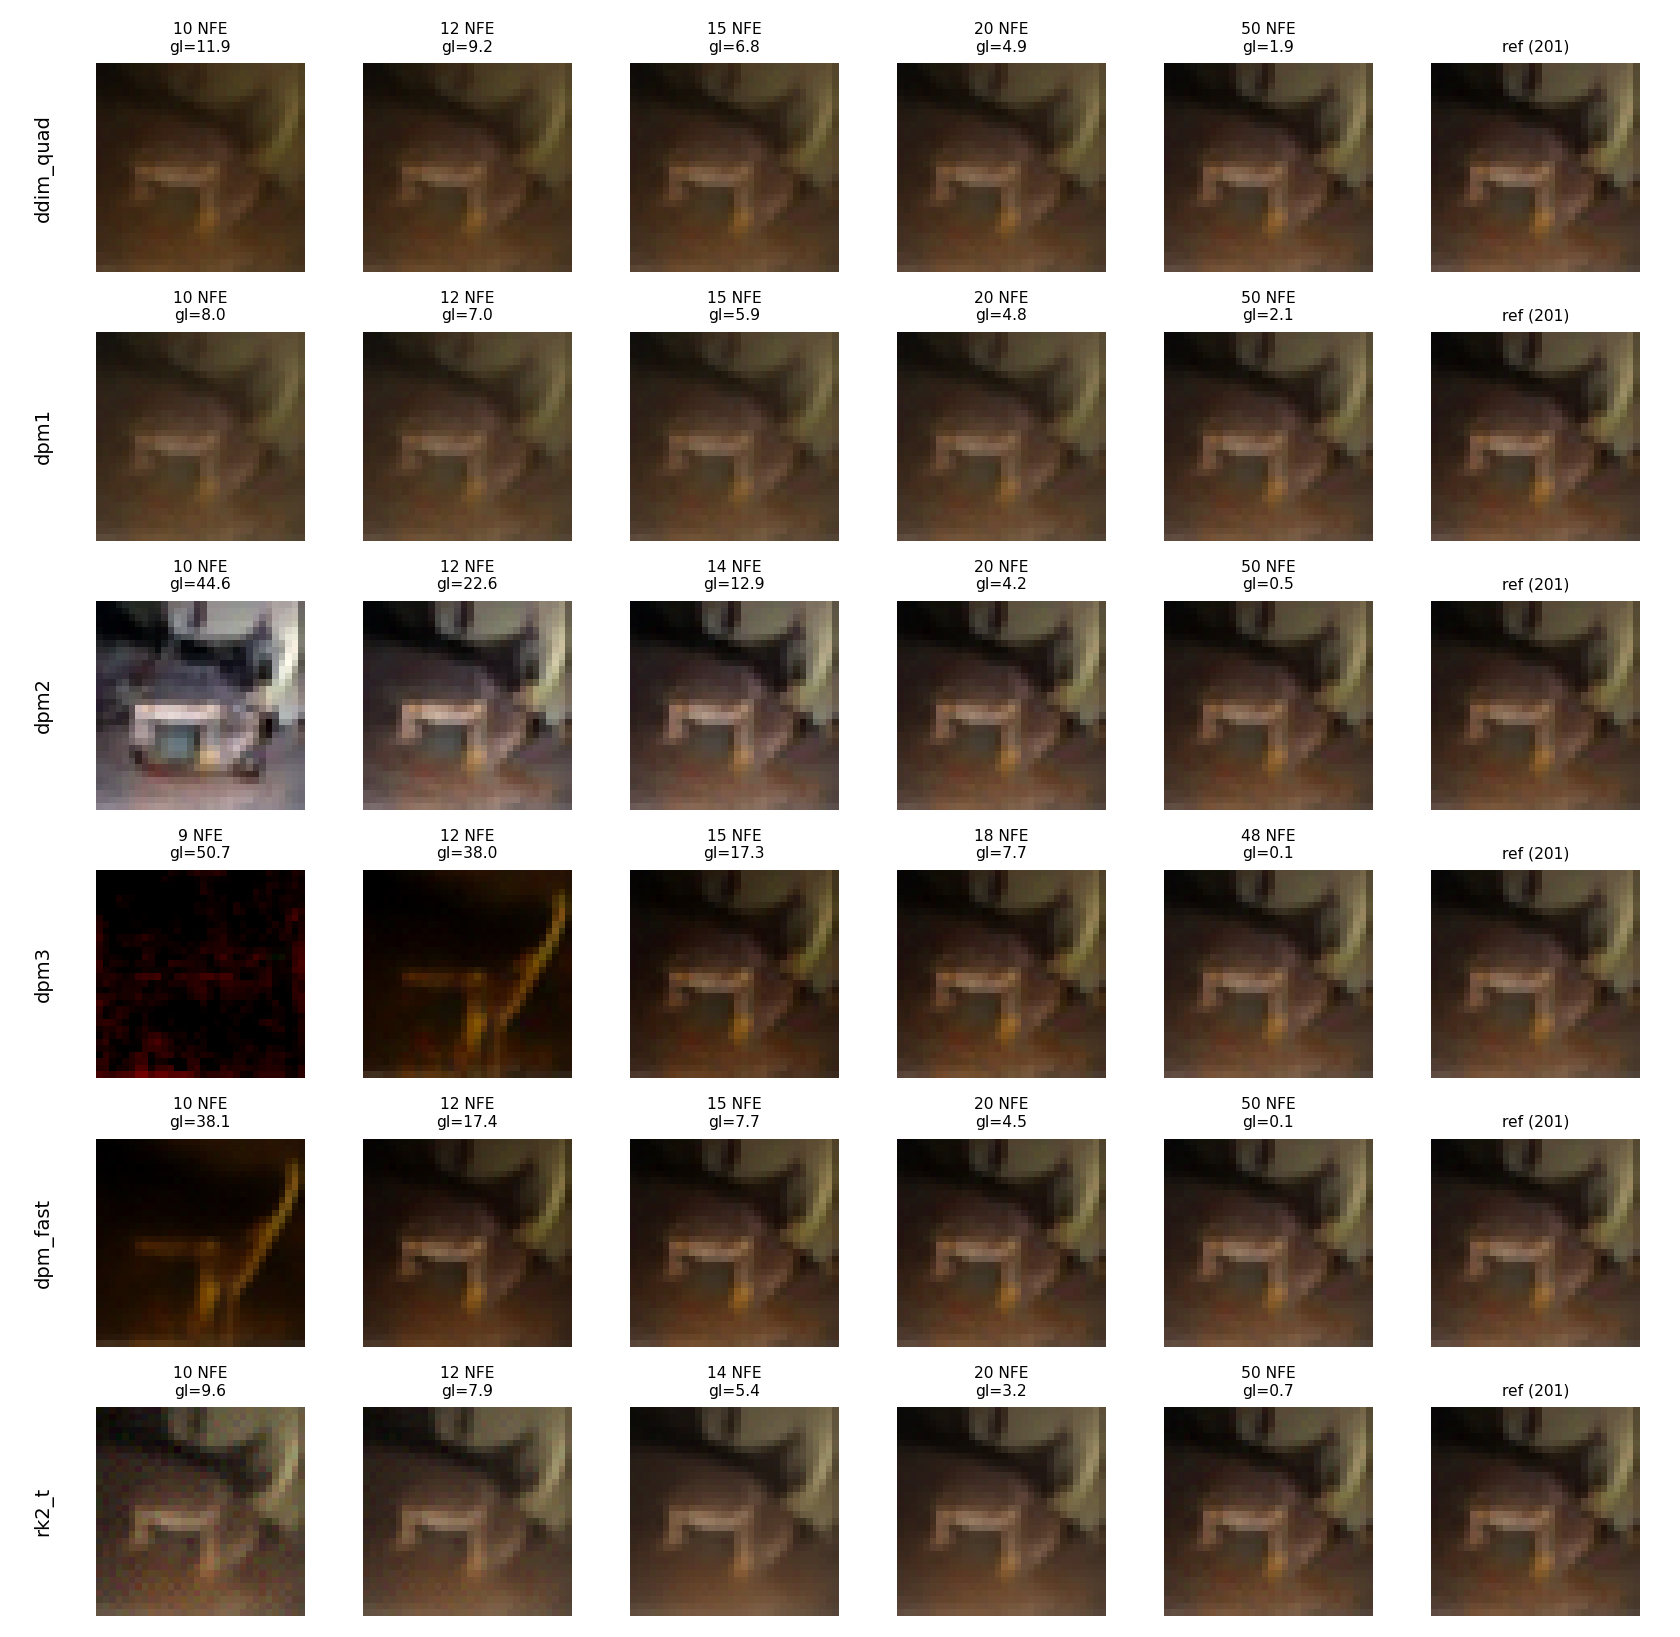
\includegraphics[width=\linewidth]{11_samples_grid.png}
\caption{One starting noise, six samplers, five budgets, and the 201-\NFE\
reference (right). ``gl'' is the mean absolute difference from the reference in
8-bit gray levels. At 10 \NFE, DDIM and DPM-Solver-1 give the right picture,
blurred; DPM-Solver-2 gives a sharp but different picture; DPM-Solver-3 at 9 \NFE\
gives noise. By 20 \NFE\ all samplers are visually close to the reference.}
\label{fig:grid}
\end{minipage}\hfill
\begin{minipage}[t]{0.47\textwidth}\vspace{0pt}\centering
\captionof{table}{Image quality and trajectory accuracy on the same checkpoint.
FID on 5,000 samples (ours) and the paper's FID (Table~6; DDIM from Table~4;
50,000 samples). $L_2$ to the converged image over 64 images, and median
per-image RMS in gray levels. DPM-$k$ is DPM-Solver-$k$.}
\label{tab:fid}
\small
\begin{tabular}{@{}lrrrrr@{}}
\toprule
Sampler & \NFE & FID & paper & $L_2$ & gray \\
\midrule
\multicolumn{6}{@{}l}{\emph{about 10 \NFE}} \\
DPM-2        & 10 & \textbf{24.9} & 7.90  & 180.6 & 49.3 \\
DPM-fast     & 10 & 31.3  & \textbf{6.42} & 111.7 & 30.2 \\
DDIM, quad.  & 10 & 39.5  & 13.58 & 91.9  & 25.8 \\
DPM-1        & 10 & 44.9  & 16.69 & 78.4  & 21.9 \\
RK2 in $t$   & 10 & 52.9  & n/a   & \textbf{44.4} & 11.3 \\
DPM-3        & 9  & 143.3 & 24.37 & 287.0 & 82.5 \\
\midrule
\multicolumn{6}{@{}l}{\emph{about 20 \NFE}} \\
DPM-2        & 20 & \textbf{15.6} & \textbf{5.24} & 27.3 & 7.1 \\
RK2 in $t$   & 20 & 15.7 & n/a  & \textbf{15.6} & 3.7 \\
DPM-fast     & 20 & 18.0 & 5.52 & 18.7 & 4.1 \\
DPM-3        & 18 & 18.7 & 5.43 & 26.4 & 6.4 \\
DDIM, quad.  & 20 & 25.1 & 6.94 & 49.8 & 13.9 \\
DPM-1        & 20 & 27.0 & 8.90 & 46.3 & 12.2 \\
\midrule
converged    & 99 & 16.5 & ${\sim}5.25$ & & \\
\bottomrule
\end{tabular}
\end{minipage}
\end{figure*}

\subsection{Samples, FID and trajectory error}
\label{sec:fid}

We rendered samples from six samplers at five budgets (Figure~\ref{fig:grid}) and
scored them with FID on 5,000 samples each, next to their $L_2$ distance to the
converged image on a 64-image batch (Table~\ref{tab:fid}).

Our FID ranking agrees with the paper's. At about 10 \NFE, order 2 beats order 1
(DPM-Solver-2 scores 24.9 against 44.9), order 3 loses to order 1 (143 against
44.9) and DPM-Solver-fast beats DDIM (31.3 against 39.5). Only the top pair is in a
different order: DPM-Solver-2 edges DPM-Solver-fast here, while the paper has the
reverse by a small margin (6.42 against 7.90). This confirms that our Tier-3 setup
reproduces the paper's setting.

Trajectory error ranks the same samplers the other way. Among the five that produce
an image at 10 \NFE, ordering by $L_2$ (RK2 in $t$, DPM-Solver-1, DDIM,
DPM-Solver-fast, DPM-Solver-2) is the exact reverse of ordering by FID, a rank
correlation of $-1.00$. DPM-Solver-2 lands $2.3$ times further from the converged
image than DPM-Solver-1 ($180.6$ against $78.4$) and scores $1.8$ times better FID.
Figure~\ref{fig:grid} shows the reason. DPM-Solver-1 produces the right picture,
blurred; DPM-Solver-2 produces a sharp picture of something different. A few large
steps at high noise fix the layout early, and DPM-Solver-2 then denoises cleanly
toward an image that is plausible but is not where this starting noise leads. FID
rewards that outcome and $L_2$ penalises it. By 20 \NFE\ the two metrics largely
agree (rank correlation $+0.60$). The evidence therefore supports the paper's claim
that DPM-Solver produces good images in 10 \NFE, while no sampler we ran integrates
the ODE accurately at that budget: the closest, RK2 in $t$, is still 11 gray levels
RMS from the converged image.

\begin{figure}[!htb]
\centering
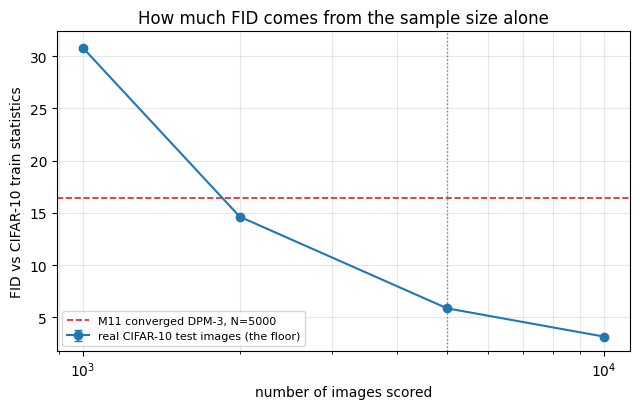
\includegraphics[width=0.82\columnwidth]{11b_fid_floor.png}
\caption{FID of real CIFAR-10 test images against sample size (three draws per
size below 10,000, the whole test set at 10,000). The dashed line is our converged DPM-Solver-3 at 5,000 samples. Real images
follow $\text{FID}\approx3.0\times10^4/N$, which sets a floor of 5.9 at our sample
size.}
\label{fig:floor}
\end{figure}

\paragraph{Absolute FID.} Our FIDs are about three times the paper's; even the
converged run scores 16.5 against about 5.25. Part of this is the sample size. Real
CIFAR-10 test images scored with the same FID call follow
$\text{FID}\approx3.0\times10^4/N$ from 1,000 to 10,000 images (Figure~\ref{fig:floor}),
and at 10,000 they give 3.15, the value documented for clean-fid, which validates the
pipeline. At our 5,000 samples the floor is 5.9; at the paper's 50,000 it is about
0.6. Sample size therefore explains 5.2 of the 11.2-point gap. The remaining 6.0
points are a real difference that we did not isolate; candidates are clean-fid's port
of the Inception network and the conversion from discrete to continuous time. The
floor shifts every sampler by the same amount, so it changes no ranking.


\subsection{Summary against the base paper and our predictions}

We wrote predictions down before running the experiments that test them: six before
any sweep, and eight more after an internal review found that an early comparison had
mixed the two protocols. The notebook \texttt{notebooks/10\_report.ipynb} computes each verdict from the results files
(Tables~\ref{tab:ledger} and~\ref{tab:ledger2}). Eleven were confirmed and three were narrowed. Stability
turned out to depend on curvature and not on $\kappa$; RK4 loses to DPM-Solver-3 per
\NFE\ only on Tier 3; and the FID sample-size floor explains about half of our gap to
the paper's absolute values.

\begin{table}[H]
\caption{Predictions made before any sweep (C: confirmed, N: narrowed).}
\label{tab:ledger}
\footnotesize
\begin{tabular}{@{}p{3.55cm}c@{\hspace{5pt}}p{3.75cm}@{}}
\toprule
Prediction & & Evidence \\
\midrule
Tiers 1, 2 slopes match theory within $\pm0.15$ & C & worst $0.094$, asymptotic protocol; up to $1.91$ at practical budgets \\
Arm A degrades as $\kappa$ grows, B and C do not & N & no $\kappa$ effect on the linear tier; RK4 limit on the curved tier \\
Euler in $\lam$ and DPM-1 both order 1, but differ & C & slopes $1.02$, $0.99$; errors differ $1.4\times$ \\
RK4 wins per step, loses per \NFE\ to DPM-3 & N & only on Tier 3 (16 to 120 \NFE); RK4 wins both on Tiers 1, 2 \\
Tier-3 slopes fall below theory & C & 8 of 9 more than $0.15$ below; mostly the budget \\
Arm B can lose to arm A at low \NFE & C & at the coarsest shared budget, all tiers \\
\bottomrule
\end{tabular}
\end{table}

\begin{table}[H]
\caption{Predictions added after the internal review.}
\label{tab:ledger2}
\footnotesize
\begin{tabular}{@{}p{3.55cm}c@{\hspace{5pt}}p{3.75cm}@{}}
\toprule
Prediction & & Evidence \\
\midrule
Exact-score tiers also miss theory at Tier 3's settings & C & worst $1.91$ against $2.79$ on Tier 3 \\
Curved tier: RK in $t$ destabilises, $\lam$ form does not & C & arm-A RK4 $h_{\max}=0.1998$; no arm-B limit \\
$\lam$ form helps RK4 on every tier at $\tend=10^{-3}$ & C & $48\times$, $8551\times$, $10.6\times$ \\
Order 3 overtakes order 1 near 10 to 12 \NFE & C & 14.1 on the paper's checkpoint \\
Exact linear part helps concentrated, hurts spread-out data & C & ahead at 83 to 100\% of points for $s<10^{-2}$; classical exact at $s=1$ \\
FID ranking at 10 \NFE\ matches Table 6 & C & headline comparisons hold; top pair swapped \\
$L_2$ and image quality disagree at low \NFE & C & rankings exactly reversed at 10 \NFE \\
Most of the FID gap is the 5k sample size & N & about half (5.2 of 11.2 points) \\
\bottomrule
\end{tabular}
\end{table}

% =====================================================================
\section{Conclusion and future work}
% =====================================================================

\subsection{Conclusions}

Measured as a numerical method, DPM-Solver behaves as its theory says wherever the
theory applies. With analytic scores and small steps every solver we tested reaches
its textbook order to within $0.1$, and the published code is correct. The order
theorem describes the limit $h\to0$, however, and at the budgets diffusion models are
sampled at (10 to 120 \NFE, down to $\tend=10^{-3}$) no solver is in that regime: exact
scores already miss theory by up to $1.9$, against $2.8$ on the network.

At those budgets two properties of the problem decide which sampler wins. The
curvature of the data distribution destabilises explicit steppers in $t$ and delays
the point where order 3 overtakes order 1, from 5 \NFE\ on a linear problem to 14 on
the real network, which reproduces the paper's Table~6 anomaly; the $\lam$
reparameterisation removes the instability and cuts RK4's error by one to four orders
of magnitude. The concentration of the data decides whether DPM-Solver's exact linear
treatment helps: it is exact for a point mass and a handicap for data as spread as the
noise.

The metric matters as well. At 10 \NFE, FID and distance to the converged image rank
samplers in opposite orders. DPM-Solver's advantage at low \NFE\ lies in producing a
plausible image, and our FID ranking agrees with the paper's; at that budget no sampler
integrates the ODE accurately. Applications that need the trajectory itself,
such as reproducible sampling, interpolation or inversion, should budget 30 to 50
\NFE: by 20 \NFE\ the two rankings largely agree, and DPM-Solver-3 comes within one
gray level of the converged image at about 36 \NFE.

\subsection{Limitations}

All Tier-3 results come from one checkpoint at $32\times32$ resolution. Our FIDs use
5,000 samples, so we compare rankings and not absolute values, and half of the gap to
the paper's absolute FIDs is unexplained. The FID samples were seeded through Python's
per-process string hash, so they are not bit-reproducible and differences of a few
tenths are noise. The Tier-3 reference is itself a numerical solution, so errors below
its floor carry no information, and the practical Tier-3 sweep is pre-asymptotic by
design. The concentration argument for natural images rests on their known covariance
spectrum, which we did not measure.

\subsection{Future work}

Natural next steps are to repeat the Tier-3 study on larger and higher-resolution
checkpoints, to compute FID on 50,000 samples with fixed seeds, to locate the
remaining FID difference by comparing the paper's original discrete-time conversion
with the interpolated schedule in the current code, to measure the pixel covariance
spectrum of CIFAR-10 to test the concentration argument directly, and to extend the
study to multistep solvers such as DPM-Solver++ and to adaptive step-size control.

\paragraph{Code availability.} The public repository
\begin{center}\url{https://github.com/MehemudAzad/NUMERICAL-PROJECT}\end{center}
contains the engine
(\texttt{src/}), 129 unit tests, one notebook per experiment, every results file and
figure, and \texttt{run\_all.sh}, which reproduces the laptop-side results from a
clean clone. The Tier-3 notebooks run on a Kaggle T4.

\bibliographystyle{ACM-Reference-Format}
\bibliography{references}

\appendix
\section{Team contributions}

\begin{itemize}
\item \textbf{Mehemud Azad} (2105014): orchestrated the team's work, put the
  members' parts together and made sure the whole pipeline runs end
  to end; planned all seven experiments (the implementation guide and the post-review
  correction plan); project setup and the shared results schema; the noise schedule
  and the $\lam\leftrightarrow t$ conversion; the Tier-1 Gaussian testbed; report
  writing: the rewrite of the technical report after the internal review, and the
  final revision of this report; the FID sample-size floor.
\item \textbf{Sayjad Rahman} (2105021): the classical steppers and the integrator
  that measures \NFE; the $\lam$-uniform grids; DPM-Solver-1 and DDIM, the wrapper
  around the authors' code and the DDIM $\equiv$ DPM-Solver-1 check; the samples and
  FID on Kaggle; the control experiments (both protocols, Tier-2 stability, the
  matched-\NFE\ crossover, when the exact linear part helps).
\item \textbf{Gourove Roy} (2105017): Tier 3 on the real network (the checkpoint's
  own schedule, the Kaggle runs and the error decomposition); the shared engine that
  runs all three tiers; the report tables and predictions ledger, and the
  floor-aware order fit; the reproduction script \texttt{run\_all.sh}; the first
  version of the technical report and this ACM-format report.
\item \textbf{Khalid Hasan Tuhin} (2105002): selected the project idea; designed
  and built the Tier-2 testbed (\texttt{mog8}, an 8-mode mixture on a Swiss roll
  whose exact score makes the probability-flow ODE nonlinear), with its DOP853
  reference and convergence check, which every Tier-2 result in the order,
  stability and crossover sections runs on; the Tier-2 convergence experiment; the
  crossover study: the crossing finder that the matched-\NFE\ crossover reuses, and
  the equal-step-size crossover on Tier 1 across five decades of $\kappa$ and on
  Tier 2.
\item \textbf{Niloy Das Robin} (2105019): the order-measurement and stability
  tools, and the Tier-1 studies built on them.

  \smallskip\noindent \emph{Order.} The sliding-window order fitter, which finds the asymptotic part
  of a convergence curve on its own and reports the slope, fit window and $R^2$;
  the Tier-1 convergence experiment over all fourteen solvers in the three arms
  (Section~\ref{sec:order}, Figure~\ref{fig:errh}).

  \smallskip\noindent \emph{Stability.} The divergence test and the bisection for the largest stable
  step, validated against a linear ODE with a known stability threshold; the
  $\kappa$-sweep stability study, with a stress test to $\kappa=10^8$ and
  $\tend=10^{-6}$.

  \smallskip\noindent \emph{Analysis.} The explanation of why the linear testbed never destabilises:
  the stability product $h\,J(\tend+h)$ stays below about 0.9, under explicit
  Euler's threshold of 2 (Section~\ref{sec:stability}).
\end{itemize}

\end{document}
